\documentclass[a4,11pt,dvipsnames]{report}
\usepackage[utf8]{inputenc}
% \usepackage[T2A]{fontenc}
\usepackage[english, russian]{babel}
% \usepackage{eufrak}
\usepackage{xltxtra}
\usepackage{polyglossia}
\usepackage{mathpazo}
\usepackage{fontspec}

\defaultfontfeatures{Ligatures=TeX,Mapping=tex-text}

\setmainfont[
ExternalLocation={/home/vyacheslav/builds/STIXv2.0.2/OTF/},
BoldFont=STIX2Text-Bold.otf,
ItalicFont=STIX2Text-Italic.otf,
BoldItalicFont=STIX2Text-BoldItalic.otf
]
{STIX2Text-Regular.otf}
\setmathrm{STIX2Math.otf}[
ExternalLocation={/home/vyacheslav/builds/STIXv2.0.2/OTF/}
]

\usepackage{amssymb, amsthm}
\usepackage{amsmath}
\usepackage{mathtools}
\usepackage{needspace}
\usepackage{enumitem}
\usepackage{cancel}
\usepackage{fdsymbol}

% разметка страницы и колонтитул
\usepackage[left=2cm,right=2cm,top=1.5cm,bottom=1cm,bindingoffset=0cm]{geometry}
\usepackage{fancybox,fancyhdr}
\fancyhf{}
\fancyhead[R]{\thepage}
\fancyhead[L]{\rightmark}
% \fancyfoot[RO,LE]{\thesection}
\fancyfoot[C]{\leftmark}
\addtolength{\headheight}{13pt}

\pagestyle{fancy}

% Отступы
\setlength{\parindent}{3ex}
\setlength{\parskip}{3pt}

\usepackage{graphicx}
\usepackage{hyperref}
\usepackage{epstopdf}

\usepackage{import}
\usepackage{xifthen}
\usepackage{pdfpages}
\usepackage{transparent}

\newcommand{\incfig}[1]{%
    \def\svgwidth{\columnwidth}
    \import{./figures/}{#1.pdf_tex}
}

\usepackage{xifthen}
\makeatother
\def\@lecture{}%
\newcommand{\lecture}[3]{
    \ifthenelse{\isempty{#3}}{%
        \def\@lecture{Лекция #1}%
    }{%
        \def\@lecture{Лекция #1: #3}%
    }%
    \subsection*{\@lecture}
    \marginpar{\small\textsf{\mbox{#2}}}
}
\makeatletter

\usepackage{xcolor}
\definecolor{Aquamarine}{cmyk}{50, 0, 17, 100}
\definecolor{ForestGreen}{cmyk}{76, 0, 76, 45}
\definecolor{Pink}{cmyk}{0, 100, 0, 0}
\definecolor{Cyan}{cmyk}{56, 0, 0, 100}
\definecolor{Gray}{gray}{0.3}

\newcommand{\Cclass}{\mathcal{C}}
\newcommand{\Dclass}{\mathcal{D}}
\newcommand{\K}{\mathcal{K}}
\newcommand{\Z}{\mathbb{Z}}
\newcommand{\N}{\mathbb{N}}
\newcommand{\Real}{\mathbb{R}}
\newcommand{\Q}{\mathbb{Q}}
\newcommand{\Cm}{\mathbb{C}}
\newcommand{\Pm}{\mathbb{P}}
\newcommand{\ord}{\operatorname{ord}}
\newcommand{\lcm}{\operatorname{lcm}}
\newcommand{\sign}{\operatorname{sign}}

\renewcommand{\o}{o}
\renewcommand{\O}{\mathcal{O}}
\renewcommand{\le}{\leqslant}
\renewcommand{\ge}{\geqslant}

\def\mybf#1{\textbf{#1}}
\def\selectedFont#1{\textbf{#1}}
% \def\mybf#1{{\usefont{T2A}{cmr}{m}{n}\textbf{#1}}}

% \usefont{T2A}{lmr}{m}{n}
% \usepackage{gentium}
% \usepackage{CormorantGaramond}

\usepackage{mdframed}
\mdfsetup{skipabove=3pt,skipbelow=3pt}
\mdfdefinestyle{defstyle}{%
    linecolor=red,
	linewidth=3pt,rightline=false,topline=false,bottomline=false,%
    frametitlerule=false,%
    frametitlebackgroundcolor=red!0,%
    innertopmargin=4pt,innerbottommargin=4pt,innerleftmargin=7pt
    frametitlebelowskip=1pt,
    frametitleaboveskip=3pt,
}
\mdfdefinestyle{thmstyle}{%
    linecolor=cyan!100,
	linewidth=2pt,topline=false,bottomline=false,%
    frametitlerule=false,%
    frametitlebackgroundcolor=cyan!20,%
    innertopmargin=4pt,innerbottommargin=4pt,
    frametitlebelowskip=1pt,
    frametitleaboveskip=3pt,
}
\theoremstyle{definition}
\mdtheorem[style=defstyle]{defn}{Определение}

\newmdtheoremenv[nobreak=true,backgroundcolor=Aquamarine!10,linewidth=0pt,innertopmargin=0pt,innerbottommargin=7pt]{cor}{Следствие}
\newmdtheoremenv[nobreak=true,backgroundcolor=CarnationPink!20,linewidth=0pt,innertopmargin=0pt,innerbottommargin=7pt]{desc}{Описание}
\newmdtheoremenv[nobreak=true,backgroundcolor=Gray!10,linewidth=0pt,innertopmargin=0pt,innerbottommargin=7pt,font={\small}]{ex}{Пример}
% \mdtheorem[style=thmstyle]{thm}{Теорема}
\newmdtheoremenv[nobreak=false,backgroundcolor=Cyan!10,linewidth=0pt,innertopmargin=0pt,innerbottommargin=7pt]{thm}{Теорема}
\newmdtheoremenv[nobreak=true,backgroundcolor=Pink!10,linewidth=0pt,innertopmargin=0pt,innerbottommargin=7pt]{lm}{Лемма}

\theoremstyle{plain}
\newtheorem*{st}{Утверждение}
\newtheorem*{prop}{Свойства}

\theoremstyle{definition}
\newtheorem*{name}{Обозначение}

\theoremstyle{remark}
\newtheorem*{rem}{Ремарка}
\newtheorem*{com}{Комментарий}
\newtheorem*{note}{Замечание}
\newtheorem*{prac}{Упражнение}
\newtheorem*{probl}{Задача}

\usepackage{fontawesome}
\renewcommand{\proofname}{Доказательство}
\renewenvironment{proof}
{ \small \hspace{\stretch{1}}\\ \faSquareO\quad  }
{ \hspace{\stretch{1}}  \faSquare \normalsize }

%{\fontsize{50}{60}\selectfont \faLinux}

\numberwithin{ex}{section}
\numberwithin{thm}{section}
\numberwithin{equation}{section}

\def\ComplexityFont#1{\textmd{\textbf{\textsf{#1}}}}
\renewcommand{\P}{\ComplexityFont{P}}
\newcommand{\DTIME}{\ComplexityFont{Dtime}}
\newcommand{\DSpace}{\ComplexityFont{DSpace}}
\newcommand{\PSPACE}{\ComplexityFont{PSPACE}}
\newcommand{\NTIME}{\ComplexityFont{Ntime}}
\newcommand{\SAT}{\ComplexityFont{SAT}}
\newcommand{\poly}{\ComplexityFont{poly}}
\newcommand{\FACTOR}{\ComplexityFont{FACTOR}}
\newcommand{\NP}{\ComplexityFont{NP}}
\newcommand{\NPcomp}{\ComplexityFont{NP-complete}}
\newcommand{\BH}{\ComplexityFont{BH}}
\newcommand{\tP}{\widetilde{\P}}
\newcommand{\tNP}{\widetilde{\NP}}
\newcommand{\tBH}{\widetilde{\BH}}
\newcommand{\UNSAT}{{\ComplexityFont{UNSAT}}}
\newcommand{\Class}{{\ComplexityFont{C}}}
\newcommand{\CircuitSat}{{\ComplexityFont{CIRCUIT\_SAT}}}
\newcommand{\tCircuitSat}{\widetilde{{\ComplexityFont{CIRCUIT\_SAT}}}}
\newcommand{\tSAT}{\widetilde{{\ComplexityFont{SAT}}}}
\newcommand{\tThreeSAT}{\widetilde{{\ComplexityFont{3\text{-}SAT}}}}
\newcommand{\ThreeSAT}{{\ComplexityFont{3\text{-}SAT}}}
\newcommand{\kQBF}{{\ComplexityFont{QBF{\tiny k}}}}
\newcommand{\QBFk}{{\ComplexityFont{QBF{\tiny k}}}}
\newcommand{\QBF}{{\ComplexityFont{QBF}}}
\newcommand{\coC}{\ComplexityFont{co-}\mathcal{C}}
\newcommand{\coNP}{\ComplexityFont{co-NP}}
\newcommand{\PH}{\ComplexityFont{PH}}
\newcommand{\EXP}{\ComplexityFont{EXP}}
\newcommand{\Size}{\ComplexityFont{Size}}
\newcommand{\Ppoly}{\ComplexityFont{P}/\ComplexityFont{poly}}

\newcommand{\const}{\textmd{const}}

\usepackage{ upgreek }
\newcommand{\PI}{\Uppi}
\newcommand{\SIGMA}{\Upsigma}
\newcommand{\DELTA}{\Updelta}



\title{Определения и формулировки по алгебре\\Линейная алгебра\\II семестр}
\author{Тамарин Вячеслав}

\begin{document}
\maketitle
\tableofcontents
\clearpage

\chapter{Линейная алгебра}
% \documentclass[11pt,dvipsnames]{report}
% \usepackage[utf8]{inputenc}
% \usepackage[T2A]{fontenc}
\usepackage[english, russian]{babel}
% \usepackage{eufrak}
\usepackage{xltxtra}
\usepackage{polyglossia}
\usepackage{mathpazo}
\usepackage{fontspec}

\defaultfontfeatures{Ligatures=TeX,Mapping=tex-text}

\setmainfont[
ExternalLocation={/home/vyacheslav/builds/STIXv2.0.2/OTF/},
BoldFont=STIX2Text-Bold.otf,
ItalicFont=STIX2Text-Italic.otf,
BoldItalicFont=STIX2Text-BoldItalic.otf
]
{STIX2Text-Regular.otf}
\setmathrm{STIX2Math.otf}[
ExternalLocation={/home/vyacheslav/builds/STIXv2.0.2/OTF/}
]

\usepackage{amssymb, amsthm}
\usepackage{amsmath}
\usepackage{mathtools}
\usepackage{needspace}
\usepackage{enumitem}
\usepackage{cancel}
\usepackage{fdsymbol}

% разметка страницы и колонтитул
\usepackage[left=2cm,right=2cm,top=1.5cm,bottom=1cm,bindingoffset=0cm]{geometry}
\usepackage{fancybox,fancyhdr}
\fancyhf{}
\fancyhead[R]{\thepage}
\fancyhead[L]{\rightmark}
% \fancyfoot[RO,LE]{\thesection}
\fancyfoot[C]{\leftmark}
\addtolength{\headheight}{13pt}

\pagestyle{fancy}

% Отступы
\setlength{\parindent}{3ex}
\setlength{\parskip}{3pt}

\usepackage{graphicx}
\usepackage{hyperref}
\usepackage{epstopdf}

\usepackage{import}
\usepackage{xifthen}
\usepackage{pdfpages}
\usepackage{transparent}

\newcommand{\incfig}[1]{%
    \def\svgwidth{\columnwidth}
    \import{./figures/}{#1.pdf_tex}
}

\usepackage{xifthen}
\makeatother
\def\@lecture{}%
\newcommand{\lecture}[3]{
    \ifthenelse{\isempty{#3}}{%
        \def\@lecture{Лекция #1}%
    }{%
        \def\@lecture{Лекция #1: #3}%
    }%
    \subsection*{\@lecture}
    \marginpar{\small\textsf{\mbox{#2}}}
}
\makeatletter

\usepackage{xcolor}
\definecolor{Aquamarine}{cmyk}{50, 0, 17, 100}
\definecolor{ForestGreen}{cmyk}{76, 0, 76, 45}
\definecolor{Pink}{cmyk}{0, 100, 0, 0}
\definecolor{Cyan}{cmyk}{56, 0, 0, 100}
\definecolor{Gray}{gray}{0.3}

\newcommand{\Cclass}{\mathcal{C}}
\newcommand{\Dclass}{\mathcal{D}}
\newcommand{\K}{\mathcal{K}}
\newcommand{\Z}{\mathbb{Z}}
\newcommand{\N}{\mathbb{N}}
\newcommand{\Real}{\mathbb{R}}
\newcommand{\Q}{\mathbb{Q}}
\newcommand{\Cm}{\mathbb{C}}
\newcommand{\Pm}{\mathbb{P}}
\newcommand{\ord}{\operatorname{ord}}
\newcommand{\lcm}{\operatorname{lcm}}
\newcommand{\sign}{\operatorname{sign}}

\renewcommand{\o}{o}
\renewcommand{\O}{\mathcal{O}}
\renewcommand{\le}{\leqslant}
\renewcommand{\ge}{\geqslant}

\def\mybf#1{\textbf{#1}}
\def\selectedFont#1{\textbf{#1}}
% \def\mybf#1{{\usefont{T2A}{cmr}{m}{n}\textbf{#1}}}

% \usefont{T2A}{lmr}{m}{n}
% \usepackage{gentium}
% \usepackage{CormorantGaramond}

\usepackage{mdframed}
\mdfsetup{skipabove=3pt,skipbelow=3pt}
\mdfdefinestyle{defstyle}{%
    linecolor=red,
	linewidth=3pt,rightline=false,topline=false,bottomline=false,%
    frametitlerule=false,%
    frametitlebackgroundcolor=red!0,%
    innertopmargin=4pt,innerbottommargin=4pt,innerleftmargin=7pt
    frametitlebelowskip=1pt,
    frametitleaboveskip=3pt,
}
\mdfdefinestyle{thmstyle}{%
    linecolor=cyan!100,
	linewidth=2pt,topline=false,bottomline=false,%
    frametitlerule=false,%
    frametitlebackgroundcolor=cyan!20,%
    innertopmargin=4pt,innerbottommargin=4pt,
    frametitlebelowskip=1pt,
    frametitleaboveskip=3pt,
}
\theoremstyle{definition}
\mdtheorem[style=defstyle]{defn}{Определение}

\newmdtheoremenv[nobreak=true,backgroundcolor=Aquamarine!10,linewidth=0pt,innertopmargin=0pt,innerbottommargin=7pt]{cor}{Следствие}
\newmdtheoremenv[nobreak=true,backgroundcolor=CarnationPink!20,linewidth=0pt,innertopmargin=0pt,innerbottommargin=7pt]{desc}{Описание}
\newmdtheoremenv[nobreak=true,backgroundcolor=Gray!10,linewidth=0pt,innertopmargin=0pt,innerbottommargin=7pt,font={\small}]{ex}{Пример}
% \mdtheorem[style=thmstyle]{thm}{Теорема}
\newmdtheoremenv[nobreak=false,backgroundcolor=Cyan!10,linewidth=0pt,innertopmargin=0pt,innerbottommargin=7pt]{thm}{Теорема}
\newmdtheoremenv[nobreak=true,backgroundcolor=Pink!10,linewidth=0pt,innertopmargin=0pt,innerbottommargin=7pt]{lm}{Лемма}

\theoremstyle{plain}
\newtheorem*{st}{Утверждение}
\newtheorem*{prop}{Свойства}

\theoremstyle{definition}
\newtheorem*{name}{Обозначение}

\theoremstyle{remark}
\newtheorem*{rem}{Ремарка}
\newtheorem*{com}{Комментарий}
\newtheorem*{note}{Замечание}
\newtheorem*{prac}{Упражнение}
\newtheorem*{probl}{Задача}

\usepackage{fontawesome}
\renewcommand{\proofname}{Доказательство}
\renewenvironment{proof}
{ \small \hspace{\stretch{1}}\\ \faSquareO\quad  }
{ \hspace{\stretch{1}}  \faSquare \normalsize }

%{\fontsize{50}{60}\selectfont \faLinux}

\numberwithin{ex}{section}
\numberwithin{thm}{section}
\numberwithin{equation}{section}

\def\ComplexityFont#1{\textmd{\textbf{\textsf{#1}}}}
\renewcommand{\P}{\ComplexityFont{P}}
\newcommand{\DTIME}{\ComplexityFont{Dtime}}
\newcommand{\DSpace}{\ComplexityFont{DSpace}}
\newcommand{\PSPACE}{\ComplexityFont{PSPACE}}
\newcommand{\NTIME}{\ComplexityFont{Ntime}}
\newcommand{\SAT}{\ComplexityFont{SAT}}
\newcommand{\poly}{\ComplexityFont{poly}}
\newcommand{\FACTOR}{\ComplexityFont{FACTOR}}
\newcommand{\NP}{\ComplexityFont{NP}}
\newcommand{\NPcomp}{\ComplexityFont{NP-complete}}
\newcommand{\BH}{\ComplexityFont{BH}}
\newcommand{\tP}{\widetilde{\P}}
\newcommand{\tNP}{\widetilde{\NP}}
\newcommand{\tBH}{\widetilde{\BH}}
\newcommand{\UNSAT}{{\ComplexityFont{UNSAT}}}
\newcommand{\Class}{{\ComplexityFont{C}}}
\newcommand{\CircuitSat}{{\ComplexityFont{CIRCUIT\_SAT}}}
\newcommand{\tCircuitSat}{\widetilde{{\ComplexityFont{CIRCUIT\_SAT}}}}
\newcommand{\tSAT}{\widetilde{{\ComplexityFont{SAT}}}}
\newcommand{\tThreeSAT}{\widetilde{{\ComplexityFont{3\text{-}SAT}}}}
\newcommand{\ThreeSAT}{{\ComplexityFont{3\text{-}SAT}}}
\newcommand{\kQBF}{{\ComplexityFont{QBF{\tiny k}}}}
\newcommand{\QBFk}{{\ComplexityFont{QBF{\tiny k}}}}
\newcommand{\QBF}{{\ComplexityFont{QBF}}}
\newcommand{\coC}{\ComplexityFont{co-}\mathcal{C}}
\newcommand{\coNP}{\ComplexityFont{co-NP}}
\newcommand{\PH}{\ComplexityFont{PH}}
\newcommand{\EXP}{\ComplexityFont{EXP}}
\newcommand{\Size}{\ComplexityFont{Size}}
\newcommand{\Ppoly}{\ComplexityFont{P}/\ComplexityFont{poly}}

\newcommand{\const}{\textmd{const}}

\usepackage{ upgreek }
\newcommand{\PI}{\Uppi}
\newcommand{\SIGMA}{\Upsigma}
\newcommand{\DELTA}{\Updelta}


% \begin{document}
\section{Подгруппа, порожденная множеством. Явное описание. Примеры образующих в $ D_n$ и $ \GL_n(K)$. Понятие циклической группы.}

\subsection{Подгруппа, порожденная множеством}
\begin{defn}[Подгруппа, прожденная множеством]
    $ G$ --- группа, $ X \subset G$. Наименьшая группа $ H \le G$, содержащая $ X$ называется  {\sf подгруппой, порожденной $ X$}.  
    \begin{name}
        $ \langle X \rangle$.
    \end{name}
    \begin{note}
	Эта группа всегда существует и совпадает с 
	$
         \bigcap_{X \subset L \le G} L = \langle X \rangle
	$
    \end{note}
\end{defn}
\begin{st}[Явное описание порожденной подгруппы]
    \[
    \langle X \rangle = \{x_1^{\varepsilon_1}\cdot \ldots \cdot x_{n}^{\varepsilon _n} \mid x_i \in  X, ~ \varepsilon _i = \pm 1\}
    .\] 
    Для $ n = 1$ считаем, что такое произведение равно нейтральному элементу.
\end{st}
\begin{defn}[Группа, порожденная множеством]
    Группа $ G$ называется {\sf порожденной множеством } $ X$, если   $ \langle X \rangle = G$. Если $ X$ конечно, имеет место обозначение  $ G = \langle x_1, \ldots , x_{n} \rangle$. Все $ x_i$ называются  {\sf образующими} $ G$. Если для группы  $ G$ существует такой конечный набор, она называется  {\sf конечно порожденной}.    
\end{defn}
\begin{defn}[Циклическая подгруппа]
    $ G$ --- группа, $ g \in  G$. Подгруппа вида $ \langle g \rangle = \{g^{n}\mid n \in  \Z\}$ называется {\sf циклической подгруппой, порожденной $ g$}.  
\end{defn}
\begin{defn}[Циклическая группа]
    Группа $ G$ называется \textsf{циклической}, если она порождена одним элементом, то есть $ \exists g \in  G\colon G = \langle g \rangle$.
\end{defn}
\subsection{Примеры образующих в $ D_n$ и  $ \GL_n(K)$}
\paragraph{Образующие $ D_n$}
Заметим, что одним элементом эта группа порождена быть не может, так как она не абелева. 
\begin{st}
    Поворот $ f_{\varphi } $ на угол $ \varphi = \frac{2\pi}{n}$ и симметрия $ f_l$ относительно одной из разрешенных прямых. Тогда  $ \langle f_{\varphi }, f_l \rangle = D_n$.
\end{st}
\paragraph{Образующие $ \GL_n(K)$}
Здесь образующими будут матрицы элементарных преобразований: транспозиций (которые можно выразить через оставшиеся), псевдоотражения (домножение на число) и трансвекции (прибавление одной строки к другой, умноженной на число).
% \end{document}
 
% \documentclass[11pt,dvipsnames]{report}
% \usepackage[utf8]{inputenc}
% \usepackage[T2A]{fontenc}
\usepackage[english, russian]{babel}
% \usepackage{eufrak}
\usepackage{xltxtra}
\usepackage{polyglossia}
\usepackage{mathpazo}
\usepackage{fontspec}

\defaultfontfeatures{Ligatures=TeX,Mapping=tex-text}

\setmainfont[
ExternalLocation={/home/vyacheslav/builds/STIXv2.0.2/OTF/},
BoldFont=STIX2Text-Bold.otf,
ItalicFont=STIX2Text-Italic.otf,
BoldItalicFont=STIX2Text-BoldItalic.otf
]
{STIX2Text-Regular.otf}
\setmathrm{STIX2Math.otf}[
ExternalLocation={/home/vyacheslav/builds/STIXv2.0.2/OTF/}
]

\usepackage{amssymb, amsthm}
\usepackage{amsmath}
\usepackage{mathtools}
\usepackage{needspace}
\usepackage{enumitem}
\usepackage{cancel}
\usepackage{fdsymbol}

% разметка страницы и колонтитул
\usepackage[left=2cm,right=2cm,top=1.5cm,bottom=1cm,bindingoffset=0cm]{geometry}
\usepackage{fancybox,fancyhdr}
\fancyhf{}
\fancyhead[R]{\thepage}
\fancyhead[L]{\rightmark}
% \fancyfoot[RO,LE]{\thesection}
\fancyfoot[C]{\leftmark}
\addtolength{\headheight}{13pt}

\pagestyle{fancy}

% Отступы
\setlength{\parindent}{3ex}
\setlength{\parskip}{3pt}

\usepackage{graphicx}
\usepackage{hyperref}
\usepackage{epstopdf}

\usepackage{import}
\usepackage{xifthen}
\usepackage{pdfpages}
\usepackage{transparent}

\newcommand{\incfig}[1]{%
    \def\svgwidth{\columnwidth}
    \import{./figures/}{#1.pdf_tex}
}

\usepackage{xifthen}
\makeatother
\def\@lecture{}%
\newcommand{\lecture}[3]{
    \ifthenelse{\isempty{#3}}{%
        \def\@lecture{Лекция #1}%
    }{%
        \def\@lecture{Лекция #1: #3}%
    }%
    \subsection*{\@lecture}
    \marginpar{\small\textsf{\mbox{#2}}}
}
\makeatletter

\usepackage{xcolor}
\definecolor{Aquamarine}{cmyk}{50, 0, 17, 100}
\definecolor{ForestGreen}{cmyk}{76, 0, 76, 45}
\definecolor{Pink}{cmyk}{0, 100, 0, 0}
\definecolor{Cyan}{cmyk}{56, 0, 0, 100}
\definecolor{Gray}{gray}{0.3}

\newcommand{\Cclass}{\mathcal{C}}
\newcommand{\Dclass}{\mathcal{D}}
\newcommand{\K}{\mathcal{K}}
\newcommand{\Z}{\mathbb{Z}}
\newcommand{\N}{\mathbb{N}}
\newcommand{\Real}{\mathbb{R}}
\newcommand{\Q}{\mathbb{Q}}
\newcommand{\Cm}{\mathbb{C}}
\newcommand{\Pm}{\mathbb{P}}
\newcommand{\ord}{\operatorname{ord}}
\newcommand{\lcm}{\operatorname{lcm}}
\newcommand{\sign}{\operatorname{sign}}

\renewcommand{\o}{o}
\renewcommand{\O}{\mathcal{O}}
\renewcommand{\le}{\leqslant}
\renewcommand{\ge}{\geqslant}

\def\mybf#1{\textbf{#1}}
\def\selectedFont#1{\textbf{#1}}
% \def\mybf#1{{\usefont{T2A}{cmr}{m}{n}\textbf{#1}}}

% \usefont{T2A}{lmr}{m}{n}
% \usepackage{gentium}
% \usepackage{CormorantGaramond}

\usepackage{mdframed}
\mdfsetup{skipabove=3pt,skipbelow=3pt}
\mdfdefinestyle{defstyle}{%
    linecolor=red,
	linewidth=3pt,rightline=false,topline=false,bottomline=false,%
    frametitlerule=false,%
    frametitlebackgroundcolor=red!0,%
    innertopmargin=4pt,innerbottommargin=4pt,innerleftmargin=7pt
    frametitlebelowskip=1pt,
    frametitleaboveskip=3pt,
}
\mdfdefinestyle{thmstyle}{%
    linecolor=cyan!100,
	linewidth=2pt,topline=false,bottomline=false,%
    frametitlerule=false,%
    frametitlebackgroundcolor=cyan!20,%
    innertopmargin=4pt,innerbottommargin=4pt,
    frametitlebelowskip=1pt,
    frametitleaboveskip=3pt,
}
\theoremstyle{definition}
\mdtheorem[style=defstyle]{defn}{Определение}

\newmdtheoremenv[nobreak=true,backgroundcolor=Aquamarine!10,linewidth=0pt,innertopmargin=0pt,innerbottommargin=7pt]{cor}{Следствие}
\newmdtheoremenv[nobreak=true,backgroundcolor=CarnationPink!20,linewidth=0pt,innertopmargin=0pt,innerbottommargin=7pt]{desc}{Описание}
\newmdtheoremenv[nobreak=true,backgroundcolor=Gray!10,linewidth=0pt,innertopmargin=0pt,innerbottommargin=7pt,font={\small}]{ex}{Пример}
% \mdtheorem[style=thmstyle]{thm}{Теорема}
\newmdtheoremenv[nobreak=false,backgroundcolor=Cyan!10,linewidth=0pt,innertopmargin=0pt,innerbottommargin=7pt]{thm}{Теорема}
\newmdtheoremenv[nobreak=true,backgroundcolor=Pink!10,linewidth=0pt,innertopmargin=0pt,innerbottommargin=7pt]{lm}{Лемма}

\theoremstyle{plain}
\newtheorem*{st}{Утверждение}
\newtheorem*{prop}{Свойства}

\theoremstyle{definition}
\newtheorem*{name}{Обозначение}

\theoremstyle{remark}
\newtheorem*{rem}{Ремарка}
\newtheorem*{com}{Комментарий}
\newtheorem*{note}{Замечание}
\newtheorem*{prac}{Упражнение}
\newtheorem*{probl}{Задача}

\usepackage{fontawesome}
\renewcommand{\proofname}{Доказательство}
\renewenvironment{proof}
{ \small \hspace{\stretch{1}}\\ \faSquareO\quad  }
{ \hspace{\stretch{1}}  \faSquare \normalsize }

%{\fontsize{50}{60}\selectfont \faLinux}

\numberwithin{ex}{section}
\numberwithin{thm}{section}
\numberwithin{equation}{section}

\def\ComplexityFont#1{\textmd{\textbf{\textsf{#1}}}}
\renewcommand{\P}{\ComplexityFont{P}}
\newcommand{\DTIME}{\ComplexityFont{Dtime}}
\newcommand{\DSpace}{\ComplexityFont{DSpace}}
\newcommand{\PSPACE}{\ComplexityFont{PSPACE}}
\newcommand{\NTIME}{\ComplexityFont{Ntime}}
\newcommand{\SAT}{\ComplexityFont{SAT}}
\newcommand{\poly}{\ComplexityFont{poly}}
\newcommand{\FACTOR}{\ComplexityFont{FACTOR}}
\newcommand{\NP}{\ComplexityFont{NP}}
\newcommand{\NPcomp}{\ComplexityFont{NP-complete}}
\newcommand{\BH}{\ComplexityFont{BH}}
\newcommand{\tP}{\widetilde{\P}}
\newcommand{\tNP}{\widetilde{\NP}}
\newcommand{\tBH}{\widetilde{\BH}}
\newcommand{\UNSAT}{{\ComplexityFont{UNSAT}}}
\newcommand{\Class}{{\ComplexityFont{C}}}
\newcommand{\CircuitSat}{{\ComplexityFont{CIRCUIT\_SAT}}}
\newcommand{\tCircuitSat}{\widetilde{{\ComplexityFont{CIRCUIT\_SAT}}}}
\newcommand{\tSAT}{\widetilde{{\ComplexityFont{SAT}}}}
\newcommand{\tThreeSAT}{\widetilde{{\ComplexityFont{3\text{-}SAT}}}}
\newcommand{\ThreeSAT}{{\ComplexityFont{3\text{-}SAT}}}
\newcommand{\kQBF}{{\ComplexityFont{QBF{\tiny k}}}}
\newcommand{\QBFk}{{\ComplexityFont{QBF{\tiny k}}}}
\newcommand{\QBF}{{\ComplexityFont{QBF}}}
\newcommand{\coC}{\ComplexityFont{co-}\mathcal{C}}
\newcommand{\coNP}{\ComplexityFont{co-NP}}
\newcommand{\PH}{\ComplexityFont{PH}}
\newcommand{\EXP}{\ComplexityFont{EXP}}
\newcommand{\Size}{\ComplexityFont{Size}}
\newcommand{\Ppoly}{\ComplexityFont{P}/\ComplexityFont{poly}}

\newcommand{\const}{\textmd{const}}

\usepackage{ upgreek }
\newcommand{\PI}{\Uppi}
\newcommand{\SIGMA}{\Upsigma}
\newcommand{\DELTA}{\Updelta}


% \begin{document}
\section{Определитель как форма объема. Формы объема, связанные с выбором базиса и их свойства.}
\begin{defn}[Форма объема]
    Пусть $ n = \dim V$. Антисимметричная полилинейная форма  $ w \colon  V^{n} \to K$   называется {\sf формой объема} на $ V$. Если такая форма не равна 0, то будем говорить, что она  {\sf невырожденная}.   
\end{defn}
\begin{defn}[Определитель]
    {\sf Определителем $ \det$} называется отображение $ \det \colon M_n(K) \to  K$ такое, что
    \[
	\det (A) = \sum_{\sigma \in S_{n} }^{}\sgn(\sigma ) \prod_{1 \le i \le n} a_{i\sigma (i)}
    .\] 
\end{defn}
\begin{defn}
    Пусть $ e_1, \ldots e_n$ --- базис пространства $ V$. Определим отображение  $ \Vol_e\colon V^{n} \to  K$ такое, что 
    \[
	\Vol_e (v_1, \ldots v_n) = \det(e(v_1), \ldots , e(v_n))
    ,\] 
    где $ e\colon V \to  K^{n}$ --- отображение сопоставления координат.
\end{defn}

\begin{thm}[Свойства форм]
    \begin{enumerate}[noitemsep]
        \item Определитель является формой объема на $ K^{n}$, при этом $ \det E = 1$.
	\item Если  $ V$ --- пространство размерности  $ n$, то любая форма объема на  $ V$ имеет вид 
	     \[
		 w = w(e_1, \ldots e_n)\Vol_e
	    .\] 
	    В частности, если $ e, f$ --- базисы, то  $ \Vol_f = \det(C_{f \to  e}) \Vol_e$.
	\item Пространство форм объема одномерно.
	\item Для любой невырожденной формы объема $ w$ верно утверждение:
	     \[
		 w(v_1, \ldots v_n) = 0 \Longleftrightarrow v_1, \ldots v_n \text{ линейно зависимы}
	    .\] 
    \end{enumerate} 
\end{thm}
% \end{document}
 
\section{Ввод-вывод в С++}
\begin{itemize}[noitemsep]
    \item иерархия классов
    \item методы/флаги/манипуляторы
    \item обработка ошибок
    \item ввод-вывод пользовательских типов
\end{itemize}

\subsection{Иерархия классов}

\begin{center}
  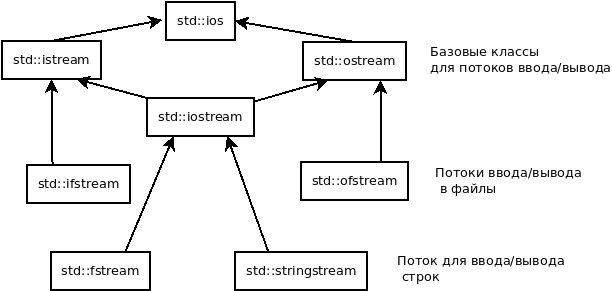
\includegraphics[width=0.8\textwidth]{io_classes.png}
\end{center}

Глобальные переенные \texttt{cin} (istream), \texttt{cout} (ostream), \texttt{cerr} (ostream).

Стандартная библиотека содержит перегруженные операторы \texttt{operator >>}, \texttt{operator <<} для примитивных типов и строк. 

\begin{minted}[fontsize=\footnotesize,numbersep=3pt,framesep=1mm,linenos,frame=single,label=]{cpp}
std::ostream& operator << (std::ostream& os, int v) {
    // convert int to bytes, write bytes
    return os;
}
\end{minted}
\begin{minted}[fontsize=\footnotesize,numbersep=3pt,framesep=1mm,linenos,frame=single,label=]{cpp}
std::istream& operator >> (std::istream& is, int& v) {
    // read bytes, convert to int
    return is;
}
\end{minted}
Такой код приводит к очистке буфера fflush потока, что замедляет вывод:
\begin{minted}[fontsize=\footnotesize,numbersep=3pt,framesep=1mm,linenos,frame=single,label=]{cpp}
std::cout << x << std::endl;
\end{minted}
Оператор читает строку до пробела, getline до конца строки:
\begin{minted}[fontsize=\footnotesize,numbersep=3pt,framesep=1mm,linenos,frame=single,label=]{cpp}
std::ifstream ifstream if("in.txt");
std::string word;
if >> word;
std::string line;
getline(if, line);
\end{minted}
Побайтовый ввод/вывод: read, write, seekg, tellg.

\subsection{Обработка ошибок}
rdstate() --- чем закончиласть последняя операция: eofbit, goodbit, failbit (считываем другим типом), badbit (не существует файла)
\subsection{Формат вывода}
\begin{minted}[fontsize=\footnotesize,numbersep=3pt,framesep=1mm,linenos,frame=single,label=]{cpp}
int x = 255;
std::cout.setf(std::ios::hex, std::ios::basefield);
std::cout << x; // после вывода флаг очистится
\end{minted}
Через манипуляторы
\begin{minted}[fontsize=\footnotesize,numbersep=3pt,framesep=1mm,linenos,frame=single,label=]{cpp}
ostream& operator << (ostream& (*pf)(ostream&));
\end{minted}
\subsection{Ввод-вывод пользовательских типов}
\begin{minted}[fontsize=\footnotesize,numbersep=3pt,framesep=1mm,linenos,frame=single,label=]{cpp}
class Point {
private:
    int x;
    int y;
public:
    friend ostream& operator << (ostream& os, const Point& p);
    friend istream& operator << (istream& is, Point& p);
    // friend функция может иметь доступ к приватным членам
};

ostream& operator << (ostream& os, const Point& p) {
    os << p.x << " " << p.y << "\n";
    return os;
}
istream& operator << (istream& is, Point& p) {
    is >> p.x >> p.y;
    return is;
}
\end{minted}
Так как ostream --- базовый класс, можно использовать один и тот же оператор для вывода на экран, строку и файл:
(cout, ofstream of("file"), stringstream ss).

 
% \documentclass[11pt,dvipsnames]{report}
% \usepackage[utf8]{inputenc}
% \usepackage[T2A]{fontenc}
\usepackage[english, russian]{babel}
% \usepackage{eufrak}
\usepackage{xltxtra}
\usepackage{polyglossia}
\usepackage{mathpazo}
\usepackage{fontspec}

\defaultfontfeatures{Ligatures=TeX,Mapping=tex-text}

\setmainfont[
ExternalLocation={/home/vyacheslav/builds/STIXv2.0.2/OTF/},
BoldFont=STIX2Text-Bold.otf,
ItalicFont=STIX2Text-Italic.otf,
BoldItalicFont=STIX2Text-BoldItalic.otf
]
{STIX2Text-Regular.otf}
\setmathrm{STIX2Math.otf}[
ExternalLocation={/home/vyacheslav/builds/STIXv2.0.2/OTF/}
]

\usepackage{amssymb, amsthm}
\usepackage{amsmath}
\usepackage{mathtools}
\usepackage{needspace}
\usepackage{enumitem}
\usepackage{cancel}
\usepackage{fdsymbol}

% разметка страницы и колонтитул
\usepackage[left=2cm,right=2cm,top=1.5cm,bottom=1cm,bindingoffset=0cm]{geometry}
\usepackage{fancybox,fancyhdr}
\fancyhf{}
\fancyhead[R]{\thepage}
\fancyhead[L]{\rightmark}
% \fancyfoot[RO,LE]{\thesection}
\fancyfoot[C]{\leftmark}
\addtolength{\headheight}{13pt}

\pagestyle{fancy}

% Отступы
\setlength{\parindent}{3ex}
\setlength{\parskip}{3pt}

\usepackage{graphicx}
\usepackage{hyperref}
\usepackage{epstopdf}

\usepackage{import}
\usepackage{xifthen}
\usepackage{pdfpages}
\usepackage{transparent}

\newcommand{\incfig}[1]{%
    \def\svgwidth{\columnwidth}
    \import{./figures/}{#1.pdf_tex}
}

\usepackage{xifthen}
\makeatother
\def\@lecture{}%
\newcommand{\lecture}[3]{
    \ifthenelse{\isempty{#3}}{%
        \def\@lecture{Лекция #1}%
    }{%
        \def\@lecture{Лекция #1: #3}%
    }%
    \subsection*{\@lecture}
    \marginpar{\small\textsf{\mbox{#2}}}
}
\makeatletter

\usepackage{xcolor}
\definecolor{Aquamarine}{cmyk}{50, 0, 17, 100}
\definecolor{ForestGreen}{cmyk}{76, 0, 76, 45}
\definecolor{Pink}{cmyk}{0, 100, 0, 0}
\definecolor{Cyan}{cmyk}{56, 0, 0, 100}
\definecolor{Gray}{gray}{0.3}

\newcommand{\Cclass}{\mathcal{C}}
\newcommand{\Dclass}{\mathcal{D}}
\newcommand{\K}{\mathcal{K}}
\newcommand{\Z}{\mathbb{Z}}
\newcommand{\N}{\mathbb{N}}
\newcommand{\Real}{\mathbb{R}}
\newcommand{\Q}{\mathbb{Q}}
\newcommand{\Cm}{\mathbb{C}}
\newcommand{\Pm}{\mathbb{P}}
\newcommand{\ord}{\operatorname{ord}}
\newcommand{\lcm}{\operatorname{lcm}}
\newcommand{\sign}{\operatorname{sign}}

\renewcommand{\o}{o}
\renewcommand{\O}{\mathcal{O}}
\renewcommand{\le}{\leqslant}
\renewcommand{\ge}{\geqslant}

\def\mybf#1{\textbf{#1}}
\def\selectedFont#1{\textbf{#1}}
% \def\mybf#1{{\usefont{T2A}{cmr}{m}{n}\textbf{#1}}}

% \usefont{T2A}{lmr}{m}{n}
% \usepackage{gentium}
% \usepackage{CormorantGaramond}

\usepackage{mdframed}
\mdfsetup{skipabove=3pt,skipbelow=3pt}
\mdfdefinestyle{defstyle}{%
    linecolor=red,
	linewidth=3pt,rightline=false,topline=false,bottomline=false,%
    frametitlerule=false,%
    frametitlebackgroundcolor=red!0,%
    innertopmargin=4pt,innerbottommargin=4pt,innerleftmargin=7pt
    frametitlebelowskip=1pt,
    frametitleaboveskip=3pt,
}
\mdfdefinestyle{thmstyle}{%
    linecolor=cyan!100,
	linewidth=2pt,topline=false,bottomline=false,%
    frametitlerule=false,%
    frametitlebackgroundcolor=cyan!20,%
    innertopmargin=4pt,innerbottommargin=4pt,
    frametitlebelowskip=1pt,
    frametitleaboveskip=3pt,
}
\theoremstyle{definition}
\mdtheorem[style=defstyle]{defn}{Определение}

\newmdtheoremenv[nobreak=true,backgroundcolor=Aquamarine!10,linewidth=0pt,innertopmargin=0pt,innerbottommargin=7pt]{cor}{Следствие}
\newmdtheoremenv[nobreak=true,backgroundcolor=CarnationPink!20,linewidth=0pt,innertopmargin=0pt,innerbottommargin=7pt]{desc}{Описание}
\newmdtheoremenv[nobreak=true,backgroundcolor=Gray!10,linewidth=0pt,innertopmargin=0pt,innerbottommargin=7pt,font={\small}]{ex}{Пример}
% \mdtheorem[style=thmstyle]{thm}{Теорема}
\newmdtheoremenv[nobreak=false,backgroundcolor=Cyan!10,linewidth=0pt,innertopmargin=0pt,innerbottommargin=7pt]{thm}{Теорема}
\newmdtheoremenv[nobreak=true,backgroundcolor=Pink!10,linewidth=0pt,innertopmargin=0pt,innerbottommargin=7pt]{lm}{Лемма}

\theoremstyle{plain}
\newtheorem*{st}{Утверждение}
\newtheorem*{prop}{Свойства}

\theoremstyle{definition}
\newtheorem*{name}{Обозначение}

\theoremstyle{remark}
\newtheorem*{rem}{Ремарка}
\newtheorem*{com}{Комментарий}
\newtheorem*{note}{Замечание}
\newtheorem*{prac}{Упражнение}
\newtheorem*{probl}{Задача}

\usepackage{fontawesome}
\renewcommand{\proofname}{Доказательство}
\renewenvironment{proof}
{ \small \hspace{\stretch{1}}\\ \faSquareO\quad  }
{ \hspace{\stretch{1}}  \faSquare \normalsize }

%{\fontsize{50}{60}\selectfont \faLinux}

\numberwithin{ex}{section}
\numberwithin{thm}{section}
\numberwithin{equation}{section}

\def\ComplexityFont#1{\textmd{\textbf{\textsf{#1}}}}
\renewcommand{\P}{\ComplexityFont{P}}
\newcommand{\DTIME}{\ComplexityFont{Dtime}}
\newcommand{\DSpace}{\ComplexityFont{DSpace}}
\newcommand{\PSPACE}{\ComplexityFont{PSPACE}}
\newcommand{\NTIME}{\ComplexityFont{Ntime}}
\newcommand{\SAT}{\ComplexityFont{SAT}}
\newcommand{\poly}{\ComplexityFont{poly}}
\newcommand{\FACTOR}{\ComplexityFont{FACTOR}}
\newcommand{\NP}{\ComplexityFont{NP}}
\newcommand{\NPcomp}{\ComplexityFont{NP-complete}}
\newcommand{\BH}{\ComplexityFont{BH}}
\newcommand{\tP}{\widetilde{\P}}
\newcommand{\tNP}{\widetilde{\NP}}
\newcommand{\tBH}{\widetilde{\BH}}
\newcommand{\UNSAT}{{\ComplexityFont{UNSAT}}}
\newcommand{\Class}{{\ComplexityFont{C}}}
\newcommand{\CircuitSat}{{\ComplexityFont{CIRCUIT\_SAT}}}
\newcommand{\tCircuitSat}{\widetilde{{\ComplexityFont{CIRCUIT\_SAT}}}}
\newcommand{\tSAT}{\widetilde{{\ComplexityFont{SAT}}}}
\newcommand{\tThreeSAT}{\widetilde{{\ComplexityFont{3\text{-}SAT}}}}
\newcommand{\ThreeSAT}{{\ComplexityFont{3\text{-}SAT}}}
\newcommand{\kQBF}{{\ComplexityFont{QBF{\tiny k}}}}
\newcommand{\QBFk}{{\ComplexityFont{QBF{\tiny k}}}}
\newcommand{\QBF}{{\ComplexityFont{QBF}}}
\newcommand{\coC}{\ComplexityFont{co-}\mathcal{C}}
\newcommand{\coNP}{\ComplexityFont{co-NP}}
\newcommand{\PH}{\ComplexityFont{PH}}
\newcommand{\EXP}{\ComplexityFont{EXP}}
\newcommand{\Size}{\ComplexityFont{Size}}
\newcommand{\Ppoly}{\ComplexityFont{P}/\ComplexityFont{poly}}

\newcommand{\const}{\textmd{const}}

\usepackage{ upgreek }
\newcommand{\PI}{\Uppi}
\newcommand{\SIGMA}{\Upsigma}
\newcommand{\DELTA}{\Updelta}


% \begin{document}
\section{Подгруппы циклических подгрупп. Прообраз подгрупп.}
\begin{thm}
    Пусть $G $ циклическая и $ H < G$. Тогда  $ H$ тоже циклическая.\\ Более того, если $ \left| G \right|  = n$,  то $ \forall d ~ n \del d\colon \exists! H \le \Z/n\colon \left| H \right| = d$. 
\end{thm}
\begin{myproof*}
    Рассмотрим два случая.
    \begin{itemize}
	\item $ G\simeq  \Z$.
	    \begin{lm}
	        Пусть $ H$ --- подгруппа в  $ \Z$. Тогда  $H $ циклическая.
	    \end{lm}
	\item $  G \simeq \Z / n$. Рассмотрим гомоморфизм, $ \pi\colon \Z \to  \Z / n$, $ \pi(x) = \overline{x}$.
	    \begin{lm}
		Пусть $ f\colon G_1 \to  G_2$ --- гомоморфизм групп, $ H \le G_2$. Тогда $ f^{-1}(H) \le G_1$.
	    \end{lm}
	    Мы знаем, что $ H \le G = \Z /n$. По прошлой лемме $ \pi^{-1}(H) \le \Z$, поэтому $ \pi^{-1}(H)$ циклическая. Из этого следует, что и $ H$ циклическая.

	    Докажем существование и единственность подгруппы порядка  $ d$, если  $ n \del d$. Рассмотрим элемент   $ \frac{n}{d} \in  \Z /n$, его порядок равен $ d$, поэтому порожденная им группа будет иметь такой же порядок.

	    Пусть  $ H = \langle x \rangle, ~ \ord x = d$. Если отождествить этот элемент с числом,  $ d = \frac{n}{(n, x)}$. Тогда $ \frac{n}{d} = (n, x) \Longrightarrow x \del \frac{n}{d} \Longrightarrow  H \subseteq \langle \frac{n}{d} \rangle$. Кроме этого в обоих группах $ d$ элементов, следовательно, они совпали.
    \end{itemize}
\end{myproof*}
% \end{document}
 
% \documentclass[11pt,dvipsnames,a4paper]{report}
% \usepackage[utf8]{inputenc}
% \usepackage[T2A]{fontenc}
\usepackage[english, russian]{babel}
% \usepackage{eufrak}
\usepackage{xltxtra}
\usepackage{polyglossia}
\usepackage{mathpazo}
\usepackage{fontspec}

\defaultfontfeatures{Ligatures=TeX,Mapping=tex-text}

\setmainfont[
ExternalLocation={/home/vyacheslav/builds/STIXv2.0.2/OTF/},
BoldFont=STIX2Text-Bold.otf,
ItalicFont=STIX2Text-Italic.otf,
BoldItalicFont=STIX2Text-BoldItalic.otf
]
{STIX2Text-Regular.otf}
\setmathrm{STIX2Math.otf}[
ExternalLocation={/home/vyacheslav/builds/STIXv2.0.2/OTF/}
]

\usepackage{amssymb, amsthm}
\usepackage{amsmath}
\usepackage{mathtools}
\usepackage{needspace}
\usepackage{enumitem}
\usepackage{cancel}
\usepackage{fdsymbol}

% разметка страницы и колонтитул
\usepackage[left=2cm,right=2cm,top=1.5cm,bottom=1cm,bindingoffset=0cm]{geometry}
\usepackage{fancybox,fancyhdr}
\fancyhf{}
\fancyhead[R]{\thepage}
\fancyhead[L]{\rightmark}
% \fancyfoot[RO,LE]{\thesection}
\fancyfoot[C]{\leftmark}
\addtolength{\headheight}{13pt}

\pagestyle{fancy}

% Отступы
\setlength{\parindent}{3ex}
\setlength{\parskip}{3pt}

\usepackage{graphicx}
\usepackage{hyperref}
\usepackage{epstopdf}

\usepackage{import}
\usepackage{xifthen}
\usepackage{pdfpages}
\usepackage{transparent}

\newcommand{\incfig}[1]{%
    \def\svgwidth{\columnwidth}
    \import{./figures/}{#1.pdf_tex}
}

\usepackage{xifthen}
\makeatother
\def\@lecture{}%
\newcommand{\lecture}[3]{
    \ifthenelse{\isempty{#3}}{%
        \def\@lecture{Лекция #1}%
    }{%
        \def\@lecture{Лекция #1: #3}%
    }%
    \subsection*{\@lecture}
    \marginpar{\small\textsf{\mbox{#2}}}
}
\makeatletter

\usepackage{xcolor}
\definecolor{Aquamarine}{cmyk}{50, 0, 17, 100}
\definecolor{ForestGreen}{cmyk}{76, 0, 76, 45}
\definecolor{Pink}{cmyk}{0, 100, 0, 0}
\definecolor{Cyan}{cmyk}{56, 0, 0, 100}
\definecolor{Gray}{gray}{0.3}

\newcommand{\Cclass}{\mathcal{C}}
\newcommand{\Dclass}{\mathcal{D}}
\newcommand{\K}{\mathcal{K}}
\newcommand{\Z}{\mathbb{Z}}
\newcommand{\N}{\mathbb{N}}
\newcommand{\Real}{\mathbb{R}}
\newcommand{\Q}{\mathbb{Q}}
\newcommand{\Cm}{\mathbb{C}}
\newcommand{\Pm}{\mathbb{P}}
\newcommand{\ord}{\operatorname{ord}}
\newcommand{\lcm}{\operatorname{lcm}}
\newcommand{\sign}{\operatorname{sign}}

\renewcommand{\o}{o}
\renewcommand{\O}{\mathcal{O}}
\renewcommand{\le}{\leqslant}
\renewcommand{\ge}{\geqslant}

\def\mybf#1{\textbf{#1}}
\def\selectedFont#1{\textbf{#1}}
% \def\mybf#1{{\usefont{T2A}{cmr}{m}{n}\textbf{#1}}}

% \usefont{T2A}{lmr}{m}{n}
% \usepackage{gentium}
% \usepackage{CormorantGaramond}

\usepackage{mdframed}
\mdfsetup{skipabove=3pt,skipbelow=3pt}
\mdfdefinestyle{defstyle}{%
    linecolor=red,
	linewidth=3pt,rightline=false,topline=false,bottomline=false,%
    frametitlerule=false,%
    frametitlebackgroundcolor=red!0,%
    innertopmargin=4pt,innerbottommargin=4pt,innerleftmargin=7pt
    frametitlebelowskip=1pt,
    frametitleaboveskip=3pt,
}
\mdfdefinestyle{thmstyle}{%
    linecolor=cyan!100,
	linewidth=2pt,topline=false,bottomline=false,%
    frametitlerule=false,%
    frametitlebackgroundcolor=cyan!20,%
    innertopmargin=4pt,innerbottommargin=4pt,
    frametitlebelowskip=1pt,
    frametitleaboveskip=3pt,
}
\theoremstyle{definition}
\mdtheorem[style=defstyle]{defn}{Определение}

\newmdtheoremenv[nobreak=true,backgroundcolor=Aquamarine!10,linewidth=0pt,innertopmargin=0pt,innerbottommargin=7pt]{cor}{Следствие}
\newmdtheoremenv[nobreak=true,backgroundcolor=CarnationPink!20,linewidth=0pt,innertopmargin=0pt,innerbottommargin=7pt]{desc}{Описание}
\newmdtheoremenv[nobreak=true,backgroundcolor=Gray!10,linewidth=0pt,innertopmargin=0pt,innerbottommargin=7pt,font={\small}]{ex}{Пример}
% \mdtheorem[style=thmstyle]{thm}{Теорема}
\newmdtheoremenv[nobreak=false,backgroundcolor=Cyan!10,linewidth=0pt,innertopmargin=0pt,innerbottommargin=7pt]{thm}{Теорема}
\newmdtheoremenv[nobreak=true,backgroundcolor=Pink!10,linewidth=0pt,innertopmargin=0pt,innerbottommargin=7pt]{lm}{Лемма}

\theoremstyle{plain}
\newtheorem*{st}{Утверждение}
\newtheorem*{prop}{Свойства}

\theoremstyle{definition}
\newtheorem*{name}{Обозначение}

\theoremstyle{remark}
\newtheorem*{rem}{Ремарка}
\newtheorem*{com}{Комментарий}
\newtheorem*{note}{Замечание}
\newtheorem*{prac}{Упражнение}
\newtheorem*{probl}{Задача}

\usepackage{fontawesome}
\renewcommand{\proofname}{Доказательство}
\renewenvironment{proof}
{ \small \hspace{\stretch{1}}\\ \faSquareO\quad  }
{ \hspace{\stretch{1}}  \faSquare \normalsize }

%{\fontsize{50}{60}\selectfont \faLinux}

\numberwithin{ex}{section}
\numberwithin{thm}{section}
\numberwithin{equation}{section}

\def\ComplexityFont#1{\textmd{\textbf{\textsf{#1}}}}
\renewcommand{\P}{\ComplexityFont{P}}
\newcommand{\DTIME}{\ComplexityFont{Dtime}}
\newcommand{\DSpace}{\ComplexityFont{DSpace}}
\newcommand{\PSPACE}{\ComplexityFont{PSPACE}}
\newcommand{\NTIME}{\ComplexityFont{Ntime}}
\newcommand{\SAT}{\ComplexityFont{SAT}}
\newcommand{\poly}{\ComplexityFont{poly}}
\newcommand{\FACTOR}{\ComplexityFont{FACTOR}}
\newcommand{\NP}{\ComplexityFont{NP}}
\newcommand{\NPcomp}{\ComplexityFont{NP-complete}}
\newcommand{\BH}{\ComplexityFont{BH}}
\newcommand{\tP}{\widetilde{\P}}
\newcommand{\tNP}{\widetilde{\NP}}
\newcommand{\tBH}{\widetilde{\BH}}
\newcommand{\UNSAT}{{\ComplexityFont{UNSAT}}}
\newcommand{\Class}{{\ComplexityFont{C}}}
\newcommand{\CircuitSat}{{\ComplexityFont{CIRCUIT\_SAT}}}
\newcommand{\tCircuitSat}{\widetilde{{\ComplexityFont{CIRCUIT\_SAT}}}}
\newcommand{\tSAT}{\widetilde{{\ComplexityFont{SAT}}}}
\newcommand{\tThreeSAT}{\widetilde{{\ComplexityFont{3\text{-}SAT}}}}
\newcommand{\ThreeSAT}{{\ComplexityFont{3\text{-}SAT}}}
\newcommand{\kQBF}{{\ComplexityFont{QBF{\tiny k}}}}
\newcommand{\QBFk}{{\ComplexityFont{QBF{\tiny k}}}}
\newcommand{\QBF}{{\ComplexityFont{QBF}}}
\newcommand{\coC}{\ComplexityFont{co-}\mathcal{C}}
\newcommand{\coNP}{\ComplexityFont{co-NP}}
\newcommand{\PH}{\ComplexityFont{PH}}
\newcommand{\EXP}{\ComplexityFont{EXP}}
\newcommand{\Size}{\ComplexityFont{Size}}
\newcommand{\Ppoly}{\ComplexityFont{P}/\ComplexityFont{poly}}

\newcommand{\const}{\textmd{const}}

\usepackage{ upgreek }
\newcommand{\PI}{\Uppi}
\newcommand{\SIGMA}{\Upsigma}
\newcommand{\DELTA}{\Updelta}


% \begin{document}
\section{Структуры. Интрузивный связный список на C}
\begin{itemize}[noitemsep]
    \item интрузивная реализация
    \item typedef
\end{itemize}
\subsection{Интрузивная реализация}
Такой список хранит интрузивные вершины, внутри которых лежат вершины с данными. Внутренние блоки не имеют связи между собой. За счет этого мы можем создать один список и использовать его для разных типов.
\begin{ccode}
#include <stdlib.h>

struct IntrusiveNode {
    struct IntrusiveNode *next;
    struct IntrusiveNode *prev;
};

struct IntrusiveList {
    struct IntrusiveNode *head;
};

struct Node {
    int data;
    struct IntrusiveNode *node;
};

void add_intr_node(struct IntrusiveList *list, struct IntrusiveNode *new_node) {
    new_node->prev = list->head;
    new_node->next = list->head->next;
    new_node->next->prev = new_node;
    list->head->next = new_node;
}

void add_node(struct IntrusiveList *list, int data) {
    struct Node *new_node = malloc(sizeof(struct Node));
    struct IntrusiveNode *new_intr_node = malloc(sizeof(struct IntrusiveNode));
    new_node->data = data;
    new_node->node = new_intr_node;
    add_intr_node(list, new_intr_node); 
}

void delete_node(struct IntrusiveList *list, struct Node *dnode) {
    struct IntrusiveNode *intr_node = dnode->node;
    intr_node->prev->next = intr_node->next;
    intr_node->next->prev = intr_node->prev;
    free(dnode); free(intr_node);
}
\end{ccode}
\subsection{typedef}
Не команда для препроцессора, это просто синоним для существующего типа.
\begin{ccode}
typedef long long ll;
typedef struct point {
    //pass
} point_s
\end{ccode}
% \end{document}
 
\section{Формула для обратной матрицы. Присоединенная матрица. Соотношение для присоединенной матрицы.}
\begin{defn}[Присоединенная матрица]
{\sf Присоединенная матрица} к матрице $ A$ --- матрица $ (\Adj A)_{ij} = A^{ij}$, где $ A^{ij}$ --- алгебраическое дополнение элемента $ a_{ij}$.   
\end{defn}
\begin{thm}
    Пусть $ A \in M_n(K)$. Тогда 
    $
	\Adj A \cdot A = A \cdot \Adj A = \det( A) \cdot E
	$.
\end{thm}
 
% \documentclass[11pt,dvipsnames]{report}
% \usepackage[utf8]{inputenc}
% \usepackage[T2A]{fontenc}
\usepackage[english, russian]{babel}
% \usepackage{eufrak}
\usepackage{xltxtra}
\usepackage{polyglossia}
\usepackage{mathpazo}
\usepackage{fontspec}

\defaultfontfeatures{Ligatures=TeX,Mapping=tex-text}

\setmainfont[
ExternalLocation={/home/vyacheslav/builds/STIXv2.0.2/OTF/},
BoldFont=STIX2Text-Bold.otf,
ItalicFont=STIX2Text-Italic.otf,
BoldItalicFont=STIX2Text-BoldItalic.otf
]
{STIX2Text-Regular.otf}
\setmathrm{STIX2Math.otf}[
ExternalLocation={/home/vyacheslav/builds/STIXv2.0.2/OTF/}
]

\usepackage{amssymb, amsthm}
\usepackage{amsmath}
\usepackage{mathtools}
\usepackage{needspace}
\usepackage{enumitem}
\usepackage{cancel}
\usepackage{fdsymbol}

% разметка страницы и колонтитул
\usepackage[left=2cm,right=2cm,top=1.5cm,bottom=1cm,bindingoffset=0cm]{geometry}
\usepackage{fancybox,fancyhdr}
\fancyhf{}
\fancyhead[R]{\thepage}
\fancyhead[L]{\rightmark}
% \fancyfoot[RO,LE]{\thesection}
\fancyfoot[C]{\leftmark}
\addtolength{\headheight}{13pt}

\pagestyle{fancy}

% Отступы
\setlength{\parindent}{3ex}
\setlength{\parskip}{3pt}

\usepackage{graphicx}
\usepackage{hyperref}
\usepackage{epstopdf}

\usepackage{import}
\usepackage{xifthen}
\usepackage{pdfpages}
\usepackage{transparent}

\newcommand{\incfig}[1]{%
    \def\svgwidth{\columnwidth}
    \import{./figures/}{#1.pdf_tex}
}

\usepackage{xifthen}
\makeatother
\def\@lecture{}%
\newcommand{\lecture}[3]{
    \ifthenelse{\isempty{#3}}{%
        \def\@lecture{Лекция #1}%
    }{%
        \def\@lecture{Лекция #1: #3}%
    }%
    \subsection*{\@lecture}
    \marginpar{\small\textsf{\mbox{#2}}}
}
\makeatletter

\usepackage{xcolor}
\definecolor{Aquamarine}{cmyk}{50, 0, 17, 100}
\definecolor{ForestGreen}{cmyk}{76, 0, 76, 45}
\definecolor{Pink}{cmyk}{0, 100, 0, 0}
\definecolor{Cyan}{cmyk}{56, 0, 0, 100}
\definecolor{Gray}{gray}{0.3}

\newcommand{\Cclass}{\mathcal{C}}
\newcommand{\Dclass}{\mathcal{D}}
\newcommand{\K}{\mathcal{K}}
\newcommand{\Z}{\mathbb{Z}}
\newcommand{\N}{\mathbb{N}}
\newcommand{\Real}{\mathbb{R}}
\newcommand{\Q}{\mathbb{Q}}
\newcommand{\Cm}{\mathbb{C}}
\newcommand{\Pm}{\mathbb{P}}
\newcommand{\ord}{\operatorname{ord}}
\newcommand{\lcm}{\operatorname{lcm}}
\newcommand{\sign}{\operatorname{sign}}

\renewcommand{\o}{o}
\renewcommand{\O}{\mathcal{O}}
\renewcommand{\le}{\leqslant}
\renewcommand{\ge}{\geqslant}

\def\mybf#1{\textbf{#1}}
\def\selectedFont#1{\textbf{#1}}
% \def\mybf#1{{\usefont{T2A}{cmr}{m}{n}\textbf{#1}}}

% \usefont{T2A}{lmr}{m}{n}
% \usepackage{gentium}
% \usepackage{CormorantGaramond}

\usepackage{mdframed}
\mdfsetup{skipabove=3pt,skipbelow=3pt}
\mdfdefinestyle{defstyle}{%
    linecolor=red,
	linewidth=3pt,rightline=false,topline=false,bottomline=false,%
    frametitlerule=false,%
    frametitlebackgroundcolor=red!0,%
    innertopmargin=4pt,innerbottommargin=4pt,innerleftmargin=7pt
    frametitlebelowskip=1pt,
    frametitleaboveskip=3pt,
}
\mdfdefinestyle{thmstyle}{%
    linecolor=cyan!100,
	linewidth=2pt,topline=false,bottomline=false,%
    frametitlerule=false,%
    frametitlebackgroundcolor=cyan!20,%
    innertopmargin=4pt,innerbottommargin=4pt,
    frametitlebelowskip=1pt,
    frametitleaboveskip=3pt,
}
\theoremstyle{definition}
\mdtheorem[style=defstyle]{defn}{Определение}

\newmdtheoremenv[nobreak=true,backgroundcolor=Aquamarine!10,linewidth=0pt,innertopmargin=0pt,innerbottommargin=7pt]{cor}{Следствие}
\newmdtheoremenv[nobreak=true,backgroundcolor=CarnationPink!20,linewidth=0pt,innertopmargin=0pt,innerbottommargin=7pt]{desc}{Описание}
\newmdtheoremenv[nobreak=true,backgroundcolor=Gray!10,linewidth=0pt,innertopmargin=0pt,innerbottommargin=7pt,font={\small}]{ex}{Пример}
% \mdtheorem[style=thmstyle]{thm}{Теорема}
\newmdtheoremenv[nobreak=false,backgroundcolor=Cyan!10,linewidth=0pt,innertopmargin=0pt,innerbottommargin=7pt]{thm}{Теорема}
\newmdtheoremenv[nobreak=true,backgroundcolor=Pink!10,linewidth=0pt,innertopmargin=0pt,innerbottommargin=7pt]{lm}{Лемма}

\theoremstyle{plain}
\newtheorem*{st}{Утверждение}
\newtheorem*{prop}{Свойства}

\theoremstyle{definition}
\newtheorem*{name}{Обозначение}

\theoremstyle{remark}
\newtheorem*{rem}{Ремарка}
\newtheorem*{com}{Комментарий}
\newtheorem*{note}{Замечание}
\newtheorem*{prac}{Упражнение}
\newtheorem*{probl}{Задача}

\usepackage{fontawesome}
\renewcommand{\proofname}{Доказательство}
\renewenvironment{proof}
{ \small \hspace{\stretch{1}}\\ \faSquareO\quad  }
{ \hspace{\stretch{1}}  \faSquare \normalsize }

%{\fontsize{50}{60}\selectfont \faLinux}

\numberwithin{ex}{section}
\numberwithin{thm}{section}
\numberwithin{equation}{section}

\def\ComplexityFont#1{\textmd{\textbf{\textsf{#1}}}}
\renewcommand{\P}{\ComplexityFont{P}}
\newcommand{\DTIME}{\ComplexityFont{Dtime}}
\newcommand{\DSpace}{\ComplexityFont{DSpace}}
\newcommand{\PSPACE}{\ComplexityFont{PSPACE}}
\newcommand{\NTIME}{\ComplexityFont{Ntime}}
\newcommand{\SAT}{\ComplexityFont{SAT}}
\newcommand{\poly}{\ComplexityFont{poly}}
\newcommand{\FACTOR}{\ComplexityFont{FACTOR}}
\newcommand{\NP}{\ComplexityFont{NP}}
\newcommand{\NPcomp}{\ComplexityFont{NP-complete}}
\newcommand{\BH}{\ComplexityFont{BH}}
\newcommand{\tP}{\widetilde{\P}}
\newcommand{\tNP}{\widetilde{\NP}}
\newcommand{\tBH}{\widetilde{\BH}}
\newcommand{\UNSAT}{{\ComplexityFont{UNSAT}}}
\newcommand{\Class}{{\ComplexityFont{C}}}
\newcommand{\CircuitSat}{{\ComplexityFont{CIRCUIT\_SAT}}}
\newcommand{\tCircuitSat}{\widetilde{{\ComplexityFont{CIRCUIT\_SAT}}}}
\newcommand{\tSAT}{\widetilde{{\ComplexityFont{SAT}}}}
\newcommand{\tThreeSAT}{\widetilde{{\ComplexityFont{3\text{-}SAT}}}}
\newcommand{\ThreeSAT}{{\ComplexityFont{3\text{-}SAT}}}
\newcommand{\kQBF}{{\ComplexityFont{QBF{\tiny k}}}}
\newcommand{\QBFk}{{\ComplexityFont{QBF{\tiny k}}}}
\newcommand{\QBF}{{\ComplexityFont{QBF}}}
\newcommand{\coC}{\ComplexityFont{co-}\mathcal{C}}
\newcommand{\coNP}{\ComplexityFont{co-NP}}
\newcommand{\PH}{\ComplexityFont{PH}}
\newcommand{\EXP}{\ComplexityFont{EXP}}
\newcommand{\Size}{\ComplexityFont{Size}}
\newcommand{\Ppoly}{\ComplexityFont{P}/\ComplexityFont{poly}}

\newcommand{\const}{\textmd{const}}

\usepackage{ upgreek }
\newcommand{\PI}{\Uppi}
\newcommand{\SIGMA}{\Upsigma}
\newcommand{\DELTA}{\Updelta}


% \begin{document}
\section{Представление перестановки в виде произведения независимых циклов. Порядок перестановки. Обратная перестановка и ее циклическая запись.}
\begin{defn}[Цикл]
    Пусть  $ \{a_1, \ldots a_k\} \subset \{1, \ldots n\}$.
    {\sf Цикл} $ (a_1, \ldots , a_k)$ --- такой элемент $ c $ из  $ S_n$, что  
    \[
	c(x) =
	\begin{cases}
	    x, & x \not\in \{a_1, \ldots a_k\}\\
	    a_{i+1}, & x = a_i \wedge 1 \le i < k\\
	    a_1, & x = a_k
	\end{cases}
    .\] 
    \begin{note}
	Порядок $ (a_1, \ldots , a_k)$ равен $ k$.
    \end{note}
\end{defn}
\begin{defn}[Неподвижная точка]
    Пусть $ \sigma \in S_{n}$. {\sf Неподвижная точка} --- такой $ x \in \{1, \ldots , n\}$, что $ \sigma (x) = x$. 
    \begin{name}
	$ \Fix(\sigma ) $ --- множество всех неподвижных точек относительно $ \sigma $.  
    \end{name}
\end{defn}
\begin{defn}[Носитель]
    {\sf Носитель перестановки $ \sigma \in  S_{n} $} --- множество $ \{1, \ldots , n\} \setminus \Fix( \sigma )$.  
    \begin{name}
        $ \supp \sigma $.
    \end{name}
\end{defn}
\begin{defn}[Независимость перестановок]
    Перестановки $\sigma _1 , \sigma _2 \in S_{n} $ называются {\sf независимыми}, если $ \supp \sigma _1 \cap \supp \sigma _2 = \varnothing$.  
    \begin{prop}
        Две независимые перестановки коммутируют.
    \end{prop}
\end{defn}
\begin{thm}[Разложение в произведение циклов]
    Пусть $ \sigma \in S_{n} $. Тогда существует единственный с точностью до порядка набор независимых циклов $ c_1, \ldots , c_k, ~ c_i \ne \id$, что $ \sigma  = c_1  \ldots c_k$.
\end{thm}
\begin{thm}[Порядок перестановки]
    Пусть $ \sigma  \in S_n$ и $ \sigma  = c_1\ldots c_k$. Обозначим $ d_i$ за длину  $ c_i$. Тогда  $ \ord \sigma  = НОК\left( d_1, \ldots d_k \right) $
\end{thm}
\begin{thm}[Обратная перестановка в циклической записи]
    Пусть $ c = (a_1, \ldots a_k)$. Тогда $ c^{-1} = (a_k, \ldots a_1)$.\\ Если $ \sigma  = c_1c_2\ldots c_s$, где $ c_i$ --- независимые циклы, то  $ \sigma^{-1} = c_1^{-1}c_2^{-1}\ldots c_s^{-1}$.
\end{thm}
% \end{document}
 
\documentclass[11pt,dvipsnames]{report}
\usepackage[utf8]{inputenc}
% \usepackage[T2A]{fontenc}
\usepackage[english, russian]{babel}
% \usepackage{eufrak}
\usepackage{xltxtra}
\usepackage{polyglossia}
\usepackage{mathpazo}
\usepackage{fontspec}

\defaultfontfeatures{Ligatures=TeX,Mapping=tex-text}

\setmainfont[
ExternalLocation={/home/vyacheslav/builds/STIXv2.0.2/OTF/},
BoldFont=STIX2Text-Bold.otf,
ItalicFont=STIX2Text-Italic.otf,
BoldItalicFont=STIX2Text-BoldItalic.otf
]
{STIX2Text-Regular.otf}
\setmathrm{STIX2Math.otf}[
ExternalLocation={/home/vyacheslav/builds/STIXv2.0.2/OTF/}
]

\usepackage{amssymb, amsthm}
\usepackage{amsmath}
\usepackage{mathtools}
\usepackage{needspace}
\usepackage{enumitem}
\usepackage{cancel}
\usepackage{fdsymbol}

% разметка страницы и колонтитул
\usepackage[left=2cm,right=2cm,top=1.5cm,bottom=1cm,bindingoffset=0cm]{geometry}
\usepackage{fancybox,fancyhdr}
\fancyhf{}
\fancyhead[R]{\thepage}
\fancyhead[L]{\rightmark}
% \fancyfoot[RO,LE]{\thesection}
\fancyfoot[C]{\leftmark}
\addtolength{\headheight}{13pt}

\pagestyle{fancy}

% Отступы
\setlength{\parindent}{3ex}
\setlength{\parskip}{3pt}

\usepackage{graphicx}
\usepackage{hyperref}
\usepackage{epstopdf}

\usepackage{import}
\usepackage{xifthen}
\usepackage{pdfpages}
\usepackage{transparent}

\newcommand{\incfig}[1]{%
    \def\svgwidth{\columnwidth}
    \import{./figures/}{#1.pdf_tex}
}

\usepackage{xifthen}
\makeatother
\def\@lecture{}%
\newcommand{\lecture}[3]{
    \ifthenelse{\isempty{#3}}{%
        \def\@lecture{Лекция #1}%
    }{%
        \def\@lecture{Лекция #1: #3}%
    }%
    \subsection*{\@lecture}
    \marginpar{\small\textsf{\mbox{#2}}}
}
\makeatletter

\usepackage{xcolor}
\definecolor{Aquamarine}{cmyk}{50, 0, 17, 100}
\definecolor{ForestGreen}{cmyk}{76, 0, 76, 45}
\definecolor{Pink}{cmyk}{0, 100, 0, 0}
\definecolor{Cyan}{cmyk}{56, 0, 0, 100}
\definecolor{Gray}{gray}{0.3}

\newcommand{\Cclass}{\mathcal{C}}
\newcommand{\Dclass}{\mathcal{D}}
\newcommand{\K}{\mathcal{K}}
\newcommand{\Z}{\mathbb{Z}}
\newcommand{\N}{\mathbb{N}}
\newcommand{\Real}{\mathbb{R}}
\newcommand{\Q}{\mathbb{Q}}
\newcommand{\Cm}{\mathbb{C}}
\newcommand{\Pm}{\mathbb{P}}
\newcommand{\ord}{\operatorname{ord}}
\newcommand{\lcm}{\operatorname{lcm}}
\newcommand{\sign}{\operatorname{sign}}

\renewcommand{\o}{o}
\renewcommand{\O}{\mathcal{O}}
\renewcommand{\le}{\leqslant}
\renewcommand{\ge}{\geqslant}

\def\mybf#1{\textbf{#1}}
\def\selectedFont#1{\textbf{#1}}
% \def\mybf#1{{\usefont{T2A}{cmr}{m}{n}\textbf{#1}}}

% \usefont{T2A}{lmr}{m}{n}
% \usepackage{gentium}
% \usepackage{CormorantGaramond}

\usepackage{mdframed}
\mdfsetup{skipabove=3pt,skipbelow=3pt}
\mdfdefinestyle{defstyle}{%
    linecolor=red,
	linewidth=3pt,rightline=false,topline=false,bottomline=false,%
    frametitlerule=false,%
    frametitlebackgroundcolor=red!0,%
    innertopmargin=4pt,innerbottommargin=4pt,innerleftmargin=7pt
    frametitlebelowskip=1pt,
    frametitleaboveskip=3pt,
}
\mdfdefinestyle{thmstyle}{%
    linecolor=cyan!100,
	linewidth=2pt,topline=false,bottomline=false,%
    frametitlerule=false,%
    frametitlebackgroundcolor=cyan!20,%
    innertopmargin=4pt,innerbottommargin=4pt,
    frametitlebelowskip=1pt,
    frametitleaboveskip=3pt,
}
\theoremstyle{definition}
\mdtheorem[style=defstyle]{defn}{Определение}

\newmdtheoremenv[nobreak=true,backgroundcolor=Aquamarine!10,linewidth=0pt,innertopmargin=0pt,innerbottommargin=7pt]{cor}{Следствие}
\newmdtheoremenv[nobreak=true,backgroundcolor=CarnationPink!20,linewidth=0pt,innertopmargin=0pt,innerbottommargin=7pt]{desc}{Описание}
\newmdtheoremenv[nobreak=true,backgroundcolor=Gray!10,linewidth=0pt,innertopmargin=0pt,innerbottommargin=7pt,font={\small}]{ex}{Пример}
% \mdtheorem[style=thmstyle]{thm}{Теорема}
\newmdtheoremenv[nobreak=false,backgroundcolor=Cyan!10,linewidth=0pt,innertopmargin=0pt,innerbottommargin=7pt]{thm}{Теорема}
\newmdtheoremenv[nobreak=true,backgroundcolor=Pink!10,linewidth=0pt,innertopmargin=0pt,innerbottommargin=7pt]{lm}{Лемма}

\theoremstyle{plain}
\newtheorem*{st}{Утверждение}
\newtheorem*{prop}{Свойства}

\theoremstyle{definition}
\newtheorem*{name}{Обозначение}

\theoremstyle{remark}
\newtheorem*{rem}{Ремарка}
\newtheorem*{com}{Комментарий}
\newtheorem*{note}{Замечание}
\newtheorem*{prac}{Упражнение}
\newtheorem*{probl}{Задача}

\usepackage{fontawesome}
\renewcommand{\proofname}{Доказательство}
\renewenvironment{proof}
{ \small \hspace{\stretch{1}}\\ \faSquareO\quad  }
{ \hspace{\stretch{1}}  \faSquare \normalsize }

%{\fontsize{50}{60}\selectfont \faLinux}

\numberwithin{ex}{section}
\numberwithin{thm}{section}
\numberwithin{equation}{section}

\def\ComplexityFont#1{\textmd{\textbf{\textsf{#1}}}}
\renewcommand{\P}{\ComplexityFont{P}}
\newcommand{\DTIME}{\ComplexityFont{Dtime}}
\newcommand{\DSpace}{\ComplexityFont{DSpace}}
\newcommand{\PSPACE}{\ComplexityFont{PSPACE}}
\newcommand{\NTIME}{\ComplexityFont{Ntime}}
\newcommand{\SAT}{\ComplexityFont{SAT}}
\newcommand{\poly}{\ComplexityFont{poly}}
\newcommand{\FACTOR}{\ComplexityFont{FACTOR}}
\newcommand{\NP}{\ComplexityFont{NP}}
\newcommand{\NPcomp}{\ComplexityFont{NP-complete}}
\newcommand{\BH}{\ComplexityFont{BH}}
\newcommand{\tP}{\widetilde{\P}}
\newcommand{\tNP}{\widetilde{\NP}}
\newcommand{\tBH}{\widetilde{\BH}}
\newcommand{\UNSAT}{{\ComplexityFont{UNSAT}}}
\newcommand{\Class}{{\ComplexityFont{C}}}
\newcommand{\CircuitSat}{{\ComplexityFont{CIRCUIT\_SAT}}}
\newcommand{\tCircuitSat}{\widetilde{{\ComplexityFont{CIRCUIT\_SAT}}}}
\newcommand{\tSAT}{\widetilde{{\ComplexityFont{SAT}}}}
\newcommand{\tThreeSAT}{\widetilde{{\ComplexityFont{3\text{-}SAT}}}}
\newcommand{\ThreeSAT}{{\ComplexityFont{3\text{-}SAT}}}
\newcommand{\kQBF}{{\ComplexityFont{QBF{\tiny k}}}}
\newcommand{\QBFk}{{\ComplexityFont{QBF{\tiny k}}}}
\newcommand{\QBF}{{\ComplexityFont{QBF}}}
\newcommand{\coC}{\ComplexityFont{co-}\mathcal{C}}
\newcommand{\coNP}{\ComplexityFont{co-NP}}
\newcommand{\PH}{\ComplexityFont{PH}}
\newcommand{\EXP}{\ComplexityFont{EXP}}
\newcommand{\Size}{\ComplexityFont{Size}}
\newcommand{\Ppoly}{\ComplexityFont{P}/\ComplexityFont{poly}}

\newcommand{\const}{\textmd{const}}

\usepackage{ upgreek }
\newcommand{\PI}{\Uppi}
\newcommand{\SIGMA}{\Upsigma}
\newcommand{\DELTA}{\Updelta}


\begin{document}
\section{Разложение в произведение транспозиций. Знак перестановки. Знак как гомоморфизм. Знак и число транспозиций в разложении.}
\begin{defn}[Транспозиция]
    Цикл вида $ (ij), ~ i \ne j$ называется {\sf транспозицией}.  
\end{defn}
\begin{st}
    Любая перестановка раскладывается в произведение транспозиций.
\end{st}
\begin{defn}[Инверсия]
    Пара $ i < j$ образует  {\sf инверсию}, если $ \sigma (i) > \sigma (j)$.  
\end{defn}
\begin{defn}[Четность и знак перестановки]
    {\sf Четность перестановки} --- четность числа инверсий $ Inv(\sigma)$ в ней.  
    \\
    {\sf Знак перестановки} --- число
    \[
	\sgn( \sigma ) = (-1)^{Inv( \sigma )} = \prod_{i>j} \frac{ \sigma (i) - \sigma (j)}{i - j}
    .\] 
\end{defn}
\end{document}
 
% \documentclass[11pt,dvipsnames]{report}
% \usepackage[utf8]{inputenc}
% \usepackage[T2A]{fontenc}
\usepackage[english, russian]{babel}
% \usepackage{eufrak}
\usepackage{xltxtra}
\usepackage{polyglossia}
\usepackage{mathpazo}
\usepackage{fontspec}

\defaultfontfeatures{Ligatures=TeX,Mapping=tex-text}

\setmainfont[
ExternalLocation={/home/vyacheslav/builds/STIXv2.0.2/OTF/},
BoldFont=STIX2Text-Bold.otf,
ItalicFont=STIX2Text-Italic.otf,
BoldItalicFont=STIX2Text-BoldItalic.otf
]
{STIX2Text-Regular.otf}
\setmathrm{STIX2Math.otf}[
ExternalLocation={/home/vyacheslav/builds/STIXv2.0.2/OTF/}
]

\usepackage{amssymb, amsthm}
\usepackage{amsmath}
\usepackage{mathtools}
\usepackage{needspace}
\usepackage{enumitem}
\usepackage{cancel}
\usepackage{fdsymbol}

% разметка страницы и колонтитул
\usepackage[left=2cm,right=2cm,top=1.5cm,bottom=1cm,bindingoffset=0cm]{geometry}
\usepackage{fancybox,fancyhdr}
\fancyhf{}
\fancyhead[R]{\thepage}
\fancyhead[L]{\rightmark}
% \fancyfoot[RO,LE]{\thesection}
\fancyfoot[C]{\leftmark}
\addtolength{\headheight}{13pt}

\pagestyle{fancy}

% Отступы
\setlength{\parindent}{3ex}
\setlength{\parskip}{3pt}

\usepackage{graphicx}
\usepackage{hyperref}
\usepackage{epstopdf}

\usepackage{import}
\usepackage{xifthen}
\usepackage{pdfpages}
\usepackage{transparent}

\newcommand{\incfig}[1]{%
    \def\svgwidth{\columnwidth}
    \import{./figures/}{#1.pdf_tex}
}

\usepackage{xifthen}
\makeatother
\def\@lecture{}%
\newcommand{\lecture}[3]{
    \ifthenelse{\isempty{#3}}{%
        \def\@lecture{Лекция #1}%
    }{%
        \def\@lecture{Лекция #1: #3}%
    }%
    \subsection*{\@lecture}
    \marginpar{\small\textsf{\mbox{#2}}}
}
\makeatletter

\usepackage{xcolor}
\definecolor{Aquamarine}{cmyk}{50, 0, 17, 100}
\definecolor{ForestGreen}{cmyk}{76, 0, 76, 45}
\definecolor{Pink}{cmyk}{0, 100, 0, 0}
\definecolor{Cyan}{cmyk}{56, 0, 0, 100}
\definecolor{Gray}{gray}{0.3}

\newcommand{\Cclass}{\mathcal{C}}
\newcommand{\Dclass}{\mathcal{D}}
\newcommand{\K}{\mathcal{K}}
\newcommand{\Z}{\mathbb{Z}}
\newcommand{\N}{\mathbb{N}}
\newcommand{\Real}{\mathbb{R}}
\newcommand{\Q}{\mathbb{Q}}
\newcommand{\Cm}{\mathbb{C}}
\newcommand{\Pm}{\mathbb{P}}
\newcommand{\ord}{\operatorname{ord}}
\newcommand{\lcm}{\operatorname{lcm}}
\newcommand{\sign}{\operatorname{sign}}

\renewcommand{\o}{o}
\renewcommand{\O}{\mathcal{O}}
\renewcommand{\le}{\leqslant}
\renewcommand{\ge}{\geqslant}

\def\mybf#1{\textbf{#1}}
\def\selectedFont#1{\textbf{#1}}
% \def\mybf#1{{\usefont{T2A}{cmr}{m}{n}\textbf{#1}}}

% \usefont{T2A}{lmr}{m}{n}
% \usepackage{gentium}
% \usepackage{CormorantGaramond}

\usepackage{mdframed}
\mdfsetup{skipabove=3pt,skipbelow=3pt}
\mdfdefinestyle{defstyle}{%
    linecolor=red,
	linewidth=3pt,rightline=false,topline=false,bottomline=false,%
    frametitlerule=false,%
    frametitlebackgroundcolor=red!0,%
    innertopmargin=4pt,innerbottommargin=4pt,innerleftmargin=7pt
    frametitlebelowskip=1pt,
    frametitleaboveskip=3pt,
}
\mdfdefinestyle{thmstyle}{%
    linecolor=cyan!100,
	linewidth=2pt,topline=false,bottomline=false,%
    frametitlerule=false,%
    frametitlebackgroundcolor=cyan!20,%
    innertopmargin=4pt,innerbottommargin=4pt,
    frametitlebelowskip=1pt,
    frametitleaboveskip=3pt,
}
\theoremstyle{definition}
\mdtheorem[style=defstyle]{defn}{Определение}

\newmdtheoremenv[nobreak=true,backgroundcolor=Aquamarine!10,linewidth=0pt,innertopmargin=0pt,innerbottommargin=7pt]{cor}{Следствие}
\newmdtheoremenv[nobreak=true,backgroundcolor=CarnationPink!20,linewidth=0pt,innertopmargin=0pt,innerbottommargin=7pt]{desc}{Описание}
\newmdtheoremenv[nobreak=true,backgroundcolor=Gray!10,linewidth=0pt,innertopmargin=0pt,innerbottommargin=7pt,font={\small}]{ex}{Пример}
% \mdtheorem[style=thmstyle]{thm}{Теорема}
\newmdtheoremenv[nobreak=false,backgroundcolor=Cyan!10,linewidth=0pt,innertopmargin=0pt,innerbottommargin=7pt]{thm}{Теорема}
\newmdtheoremenv[nobreak=true,backgroundcolor=Pink!10,linewidth=0pt,innertopmargin=0pt,innerbottommargin=7pt]{lm}{Лемма}

\theoremstyle{plain}
\newtheorem*{st}{Утверждение}
\newtheorem*{prop}{Свойства}

\theoremstyle{definition}
\newtheorem*{name}{Обозначение}

\theoremstyle{remark}
\newtheorem*{rem}{Ремарка}
\newtheorem*{com}{Комментарий}
\newtheorem*{note}{Замечание}
\newtheorem*{prac}{Упражнение}
\newtheorem*{probl}{Задача}

\usepackage{fontawesome}
\renewcommand{\proofname}{Доказательство}
\renewenvironment{proof}
{ \small \hspace{\stretch{1}}\\ \faSquareO\quad  }
{ \hspace{\stretch{1}}  \faSquare \normalsize }

%{\fontsize{50}{60}\selectfont \faLinux}

\numberwithin{ex}{section}
\numberwithin{thm}{section}
\numberwithin{equation}{section}

\def\ComplexityFont#1{\textmd{\textbf{\textsf{#1}}}}
\renewcommand{\P}{\ComplexityFont{P}}
\newcommand{\DTIME}{\ComplexityFont{Dtime}}
\newcommand{\DSpace}{\ComplexityFont{DSpace}}
\newcommand{\PSPACE}{\ComplexityFont{PSPACE}}
\newcommand{\NTIME}{\ComplexityFont{Ntime}}
\newcommand{\SAT}{\ComplexityFont{SAT}}
\newcommand{\poly}{\ComplexityFont{poly}}
\newcommand{\FACTOR}{\ComplexityFont{FACTOR}}
\newcommand{\NP}{\ComplexityFont{NP}}
\newcommand{\NPcomp}{\ComplexityFont{NP-complete}}
\newcommand{\BH}{\ComplexityFont{BH}}
\newcommand{\tP}{\widetilde{\P}}
\newcommand{\tNP}{\widetilde{\NP}}
\newcommand{\tBH}{\widetilde{\BH}}
\newcommand{\UNSAT}{{\ComplexityFont{UNSAT}}}
\newcommand{\Class}{{\ComplexityFont{C}}}
\newcommand{\CircuitSat}{{\ComplexityFont{CIRCUIT\_SAT}}}
\newcommand{\tCircuitSat}{\widetilde{{\ComplexityFont{CIRCUIT\_SAT}}}}
\newcommand{\tSAT}{\widetilde{{\ComplexityFont{SAT}}}}
\newcommand{\tThreeSAT}{\widetilde{{\ComplexityFont{3\text{-}SAT}}}}
\newcommand{\ThreeSAT}{{\ComplexityFont{3\text{-}SAT}}}
\newcommand{\kQBF}{{\ComplexityFont{QBF{\tiny k}}}}
\newcommand{\QBFk}{{\ComplexityFont{QBF{\tiny k}}}}
\newcommand{\QBF}{{\ComplexityFont{QBF}}}
\newcommand{\coC}{\ComplexityFont{co-}\mathcal{C}}
\newcommand{\coNP}{\ComplexityFont{co-NP}}
\newcommand{\PH}{\ComplexityFont{PH}}
\newcommand{\EXP}{\ComplexityFont{EXP}}
\newcommand{\Size}{\ComplexityFont{Size}}
\newcommand{\Ppoly}{\ComplexityFont{P}/\ComplexityFont{poly}}

\newcommand{\const}{\textmd{const}}

\usepackage{ upgreek }
\newcommand{\PI}{\Uppi}
\newcommand{\SIGMA}{\Upsigma}
\newcommand{\DELTA}{\Updelta}


% \begin{document}
\section{Разные способы вычисления знака перестановки. Знак обратной перестановки. Знакопеременная группа. Задача о пятнадцати.}
\begin{st}
    $ \sgn \sigma  = \sgn \sigma^{-1} $
\end{st}
\begin{st}
    Пусть $ \sigma  = c_1 \ldots c_n$, $ c_i$ --- независимые циклы. Тогда  $ \sgn \sigma = (-1)^{\text{кол-во} c_i \text{ четной длины}} = (-1)^{n-k}$, где $ k $ ---  количество орбит  $ \sigma $.
\end{st}
\begin{defn}[Знакопеременная группа]
    {\sf Знакопеременная группа }  $ A_n$ --- группа 
    \[
	A_n = \{\sigma \in \S_n \mid \sigma \text{ --- четная}\} = \ker \left( \sgn  \right) 
    .\] 
    \[
	\left| A_n \right|  = \frac{n!}{2}
    .\] 
\end{defn}

% \end{document}
 
\section{Собственные числа и собственные вектора. Характеристический многочлен и его связь с собственными числами. Вычисление характеристического многочлена сопровождающей матрицы.}
\begin{defn}[Собсвенные число и вектор]
    Пусть $ V$ --- пространство с оператором $ L$. Тогда вектор  $ 0 \ne v \in V$ называется собственным вектором с собственным числом $ \lambda $ относительно оператора $ L$, если  $ Lv = \lambda v$.
\end{defn}
\begin{defn}[Характеристический многочлен]
    {\sf Характеристический многочлен} оператора $ L$ ---  $ \chi _L(t) = \det (A - tE_n)$, где  $ A$ --- матрица  $ L$  некотором базисе.  
    \begin{note}
        Характеристический многочлен корректно определен.
    \end{note}
\end{defn}

\begin{st}
    Элемент $ \lambda \in K$ является собственным числом оператора $ L$  тогда и только тогда, когда $ \lambda $ --- корень $ \chi _L(t)$.
\end{st}
\begin{defn}[Сопровождающая матрица]
    Пусть $ f(x) \in  K[x]$ --- многочлен степени больше 1. Тогда {\sf сопровождающей матрицей} к $ f(x) = x^{n} + a_{n-1}x^{n-1} + \ldots + a_0$ называется
    \[
    \begin{pmatrix}
	0&0&\ldots &0&-a_0\\
	1&0&\ldots &0&-a_1\\
	0&1&\ldots &0&-a_2\\
	\vdots &&\ddots  &&\vdots\\
	0&0 &\ldots &1&-a_{n-1}
    \end{pmatrix}
    .\] 
\end{defn}
\begin{st}
    Характеристический многочлен сопровождающей матрицы равен $ (-1)^{n}f(t)$
\end{st}
 
% \documentclass[11pt,dvipsnames]{report}
% \usepackage[utf8]{inputenc}
% \usepackage[T2A]{fontenc}
\usepackage[english, russian]{babel}
% \usepackage{eufrak}
\usepackage{xltxtra}
\usepackage{polyglossia}
\usepackage{mathpazo}
\usepackage{fontspec}

\defaultfontfeatures{Ligatures=TeX,Mapping=tex-text}

\setmainfont[
ExternalLocation={/home/vyacheslav/builds/STIXv2.0.2/OTF/},
BoldFont=STIX2Text-Bold.otf,
ItalicFont=STIX2Text-Italic.otf,
BoldItalicFont=STIX2Text-BoldItalic.otf
]
{STIX2Text-Regular.otf}
\setmathrm{STIX2Math.otf}[
ExternalLocation={/home/vyacheslav/builds/STIXv2.0.2/OTF/}
]

\usepackage{amssymb, amsthm}
\usepackage{amsmath}
\usepackage{mathtools}
\usepackage{needspace}
\usepackage{enumitem}
\usepackage{cancel}
\usepackage{fdsymbol}

% разметка страницы и колонтитул
\usepackage[left=2cm,right=2cm,top=1.5cm,bottom=1cm,bindingoffset=0cm]{geometry}
\usepackage{fancybox,fancyhdr}
\fancyhf{}
\fancyhead[R]{\thepage}
\fancyhead[L]{\rightmark}
% \fancyfoot[RO,LE]{\thesection}
\fancyfoot[C]{\leftmark}
\addtolength{\headheight}{13pt}

\pagestyle{fancy}

% Отступы
\setlength{\parindent}{3ex}
\setlength{\parskip}{3pt}

\usepackage{graphicx}
\usepackage{hyperref}
\usepackage{epstopdf}

\usepackage{import}
\usepackage{xifthen}
\usepackage{pdfpages}
\usepackage{transparent}

\newcommand{\incfig}[1]{%
    \def\svgwidth{\columnwidth}
    \import{./figures/}{#1.pdf_tex}
}

\usepackage{xifthen}
\makeatother
\def\@lecture{}%
\newcommand{\lecture}[3]{
    \ifthenelse{\isempty{#3}}{%
        \def\@lecture{Лекция #1}%
    }{%
        \def\@lecture{Лекция #1: #3}%
    }%
    \subsection*{\@lecture}
    \marginpar{\small\textsf{\mbox{#2}}}
}
\makeatletter

\usepackage{xcolor}
\definecolor{Aquamarine}{cmyk}{50, 0, 17, 100}
\definecolor{ForestGreen}{cmyk}{76, 0, 76, 45}
\definecolor{Pink}{cmyk}{0, 100, 0, 0}
\definecolor{Cyan}{cmyk}{56, 0, 0, 100}
\definecolor{Gray}{gray}{0.3}

\newcommand{\Cclass}{\mathcal{C}}
\newcommand{\Dclass}{\mathcal{D}}
\newcommand{\K}{\mathcal{K}}
\newcommand{\Z}{\mathbb{Z}}
\newcommand{\N}{\mathbb{N}}
\newcommand{\Real}{\mathbb{R}}
\newcommand{\Q}{\mathbb{Q}}
\newcommand{\Cm}{\mathbb{C}}
\newcommand{\Pm}{\mathbb{P}}
\newcommand{\ord}{\operatorname{ord}}
\newcommand{\lcm}{\operatorname{lcm}}
\newcommand{\sign}{\operatorname{sign}}

\renewcommand{\o}{o}
\renewcommand{\O}{\mathcal{O}}
\renewcommand{\le}{\leqslant}
\renewcommand{\ge}{\geqslant}

\def\mybf#1{\textbf{#1}}
\def\selectedFont#1{\textbf{#1}}
% \def\mybf#1{{\usefont{T2A}{cmr}{m}{n}\textbf{#1}}}

% \usefont{T2A}{lmr}{m}{n}
% \usepackage{gentium}
% \usepackage{CormorantGaramond}

\usepackage{mdframed}
\mdfsetup{skipabove=3pt,skipbelow=3pt}
\mdfdefinestyle{defstyle}{%
    linecolor=red,
	linewidth=3pt,rightline=false,topline=false,bottomline=false,%
    frametitlerule=false,%
    frametitlebackgroundcolor=red!0,%
    innertopmargin=4pt,innerbottommargin=4pt,innerleftmargin=7pt
    frametitlebelowskip=1pt,
    frametitleaboveskip=3pt,
}
\mdfdefinestyle{thmstyle}{%
    linecolor=cyan!100,
	linewidth=2pt,topline=false,bottomline=false,%
    frametitlerule=false,%
    frametitlebackgroundcolor=cyan!20,%
    innertopmargin=4pt,innerbottommargin=4pt,
    frametitlebelowskip=1pt,
    frametitleaboveskip=3pt,
}
\theoremstyle{definition}
\mdtheorem[style=defstyle]{defn}{Определение}

\newmdtheoremenv[nobreak=true,backgroundcolor=Aquamarine!10,linewidth=0pt,innertopmargin=0pt,innerbottommargin=7pt]{cor}{Следствие}
\newmdtheoremenv[nobreak=true,backgroundcolor=CarnationPink!20,linewidth=0pt,innertopmargin=0pt,innerbottommargin=7pt]{desc}{Описание}
\newmdtheoremenv[nobreak=true,backgroundcolor=Gray!10,linewidth=0pt,innertopmargin=0pt,innerbottommargin=7pt,font={\small}]{ex}{Пример}
% \mdtheorem[style=thmstyle]{thm}{Теорема}
\newmdtheoremenv[nobreak=false,backgroundcolor=Cyan!10,linewidth=0pt,innertopmargin=0pt,innerbottommargin=7pt]{thm}{Теорема}
\newmdtheoremenv[nobreak=true,backgroundcolor=Pink!10,linewidth=0pt,innertopmargin=0pt,innerbottommargin=7pt]{lm}{Лемма}

\theoremstyle{plain}
\newtheorem*{st}{Утверждение}
\newtheorem*{prop}{Свойства}

\theoremstyle{definition}
\newtheorem*{name}{Обозначение}

\theoremstyle{remark}
\newtheorem*{rem}{Ремарка}
\newtheorem*{com}{Комментарий}
\newtheorem*{note}{Замечание}
\newtheorem*{prac}{Упражнение}
\newtheorem*{probl}{Задача}

\usepackage{fontawesome}
\renewcommand{\proofname}{Доказательство}
\renewenvironment{proof}
{ \small \hspace{\stretch{1}}\\ \faSquareO\quad  }
{ \hspace{\stretch{1}}  \faSquare \normalsize }

%{\fontsize{50}{60}\selectfont \faLinux}

\numberwithin{ex}{section}
\numberwithin{thm}{section}
\numberwithin{equation}{section}

\def\ComplexityFont#1{\textmd{\textbf{\textsf{#1}}}}
\renewcommand{\P}{\ComplexityFont{P}}
\newcommand{\DTIME}{\ComplexityFont{Dtime}}
\newcommand{\DSpace}{\ComplexityFont{DSpace}}
\newcommand{\PSPACE}{\ComplexityFont{PSPACE}}
\newcommand{\NTIME}{\ComplexityFont{Ntime}}
\newcommand{\SAT}{\ComplexityFont{SAT}}
\newcommand{\poly}{\ComplexityFont{poly}}
\newcommand{\FACTOR}{\ComplexityFont{FACTOR}}
\newcommand{\NP}{\ComplexityFont{NP}}
\newcommand{\NPcomp}{\ComplexityFont{NP-complete}}
\newcommand{\BH}{\ComplexityFont{BH}}
\newcommand{\tP}{\widetilde{\P}}
\newcommand{\tNP}{\widetilde{\NP}}
\newcommand{\tBH}{\widetilde{\BH}}
\newcommand{\UNSAT}{{\ComplexityFont{UNSAT}}}
\newcommand{\Class}{{\ComplexityFont{C}}}
\newcommand{\CircuitSat}{{\ComplexityFont{CIRCUIT\_SAT}}}
\newcommand{\tCircuitSat}{\widetilde{{\ComplexityFont{CIRCUIT\_SAT}}}}
\newcommand{\tSAT}{\widetilde{{\ComplexityFont{SAT}}}}
\newcommand{\tThreeSAT}{\widetilde{{\ComplexityFont{3\text{-}SAT}}}}
\newcommand{\ThreeSAT}{{\ComplexityFont{3\text{-}SAT}}}
\newcommand{\kQBF}{{\ComplexityFont{QBF{\tiny k}}}}
\newcommand{\QBFk}{{\ComplexityFont{QBF{\tiny k}}}}
\newcommand{\QBF}{{\ComplexityFont{QBF}}}
\newcommand{\coC}{\ComplexityFont{co-}\mathcal{C}}
\newcommand{\coNP}{\ComplexityFont{co-NP}}
\newcommand{\PH}{\ComplexityFont{PH}}
\newcommand{\EXP}{\ComplexityFont{EXP}}
\newcommand{\Size}{\ComplexityFont{Size}}
\newcommand{\Ppoly}{\ComplexityFont{P}/\ComplexityFont{poly}}

\newcommand{\const}{\textmd{const}}

\usepackage{ upgreek }
\newcommand{\PI}{\Uppi}
\newcommand{\SIGMA}{\Upsigma}
\newcommand{\DELTA}{\Updelta}


% \begin{document}
\section{$ S_{n} $ порождена двумя образующими. Образующие $ A_n$ --- два типа.}
\begin{st}
    Группа $ S_{n} $ порождена перестановками $ (12), (1\ldots n)$.
\end{st}
\begin{st}
    Группа $ A_n$ порождена перестановками  $ (123), \ldots (12n)$.
\end{st}

\begin{st}
    Группа $ A_n$ порождена перестановками  $ (123), (12\ldots n)$, если $ n $ нечетно, и  $ (123), (23\ldots n)$,  если четно.
\end{st}

% \end{document}
 
\section{Метапрограммирование - II}
\begin{itemize}[noitemsep]
	\item переменное число параметров в стиле C (\texttt{va\_arg, va\_list, va\_start, va\_end})
	\item variadic templates (для функций)
	\item std::function (использование)
	\item std::bind (использование)
\end{itemize}

\subsection{Переменное число аргументов в стиле С}
В функции printf первым аргументом идет шаблон, а далее любое количество аргументов. 
Для этого используются три макроса \texttt{va\_start, va\_arg, va\_end}. 
\begin{minted}[fontsize=\footnotesize,numbersep=3pt,framesep=1mm,linenos,frame=single,label=printf]{cpp}
void simple_printf(const char* fmt, ...) {
	va_list args;
	va_start(args, fmt); 
	// Макрос записывает в args адрес начала следующего за fmt параметра на стеке
	while (*fmt != '\0') {
		if (*fmt == 'd') {
			int i = va_arg(args, int); // достаем из стека переменную типа int
			// здесь выводим int с помощью putc
		}
		fmt++;
	}
	va_end(args);
}

// могут возникать труднообнаруживаемые ошибки
printf("%s", 5);
printf("%d %d", 4);
printf("%d", 4, 5);
\end{minted}

\subsection{Variadic template}
Шаблон с переменным числом аргументов, подобие рекурсии.
Для рекурсии нам нужен переход о n к n-1 элементу и база, где нужно остановится.
\begin{minted}[fontsize=\footnotesize,numbersep=3pt,framesep=1mm,linenos,frame=single,label=]{cpp}
template<typename T>
T sum(T n) { return n; }

template<typename T, typename... Args>
T sum(T n, Args... rest) { return n + sum(rest...); }

double d = sum(3, (double)4.3, 5);
\end{minted}
Многоточие будет отщипывать один аргумент, далее тот же шаблон будет применяться, пока не останется один аргумент и вызовется база.

Для данного примера компилятор сгенерирует  три функции:
\begin{minted}[fontsize=\footnotesize,numbersep=3pt,framesep=1mm,linenos,frame=single,label=]{cpp}
T sum(T, Args ...) [with T = int; Args = {double, int}];
T sum(T, Args ...) [with T = double; Args = {int}];
T sum(T, Args ...) [with T = int];
\end{minted}

\subsection{Переменное число аргументов в С++11}
С помощью variadic template можно реализовать printf так, чтобы мы получали информацию об ошибках компиляции.
\begin{minted}[fontsize=\footnotesize,numbersep=3pt,framesep=1mm,linenos,frame=single,label=]{cpp}
void printf(const char *s) {
	while (*s) {
		if (*s == '%' && *(++s) != '%')
			throw std::runtime_error("invalid format");
		std::cout << *s++;
	}
}

template<typename T, typename... Args>
void printf(const char *s, T value, Args... rest) {
	while (*s) {
		if (*s == '%' && *(++s) != '%') {
			std::cout << value;
			printf(++s, rest...);
			return;
		}
		std::cout << *s++;
	}
	throw std::logic_error("extra arguments provided to printf");
}
\end{minted}

\subsection{std::function}
Используется для создания функций на этапе компиляции.  Например, есть функция с тремя параметрами, а нам нужно вызвать ее с двумя параметрами, а третий зафиксирован. 
\begin{minted}[fontsize=\footnotesize,numbersep=3pt,framesep=1mm,linenos,frame=single,label=]{cpp}
#include <functional>
void execute(const vector<function<void ()>>& fs) { 
// здесь может лежать и функция и функтор и ламбда, главное без параметров и типа void
	for (auto& f: fs) f();
}

void simple_func() {
	cout << "simple function" << endl;
}

struct functor {
	void operator () () const {
		cout << "functor" << endl;
	}
}

int main() {
	vector<function<void ()>> x;
	x.push(simple_func);
	functor functor_instance;
	x.push_back(functor_instance);
	x.push_back([] () { cout << "lambda" << endl; });
	execute(x);
}
\end{minted}

\subsection{std::bind}
Позволяет создать обертку над функцией, уменьшив количество параметров. 
\begin{minted}[fontsize=\footnotesize,numbersep=3pt,framesep=1mm,linenos,frame=single,label=]{cpp}
#include<functional>

void show_text(const string& t) { // есть параметр
    cout << "Text: " << t << endl;
}

int main() {
	vector<function<void ()>> x;
	function<void ()> f = bind(show_text, "Hello");
	x.push_back(f);
	execute(x);
\end{minted}

\subsection{placeholder}
Есть функция с параметрами, хотим подставить первый параметр другой функции на место второго.  
\begin{minted}[fontsize=\footnotesize,numbersep=3pt,framesep=1mm,linenos,frame=single,label=]{cpp}
#include <functional>
using namespace std::placeholders;

int multiplay (int a, int b) { return a * b; }

int main() {
    auto f = bind(multiplay, 5, _1); // подставляем первый параметр из f во второй из multyplay
	cout << "out: " << f(6); // = 30
}
\end{minted}

 
% \documentclass[11pt,dvipsnames]{report}
% \usepackage[utf8]{inputenc}
% \usepackage[T2A]{fontenc}
\usepackage[english, russian]{babel}
% \usepackage{eufrak}
\usepackage{xltxtra}
\usepackage{polyglossia}
\usepackage{mathpazo}
\usepackage{fontspec}

\defaultfontfeatures{Ligatures=TeX,Mapping=tex-text}

\setmainfont[
ExternalLocation={/home/vyacheslav/builds/STIXv2.0.2/OTF/},
BoldFont=STIX2Text-Bold.otf,
ItalicFont=STIX2Text-Italic.otf,
BoldItalicFont=STIX2Text-BoldItalic.otf
]
{STIX2Text-Regular.otf}
\setmathrm{STIX2Math.otf}[
ExternalLocation={/home/vyacheslav/builds/STIXv2.0.2/OTF/}
]

\usepackage{amssymb, amsthm}
\usepackage{amsmath}
\usepackage{mathtools}
\usepackage{needspace}
\usepackage{enumitem}
\usepackage{cancel}
\usepackage{fdsymbol}

% разметка страницы и колонтитул
\usepackage[left=2cm,right=2cm,top=1.5cm,bottom=1cm,bindingoffset=0cm]{geometry}
\usepackage{fancybox,fancyhdr}
\fancyhf{}
\fancyhead[R]{\thepage}
\fancyhead[L]{\rightmark}
% \fancyfoot[RO,LE]{\thesection}
\fancyfoot[C]{\leftmark}
\addtolength{\headheight}{13pt}

\pagestyle{fancy}

% Отступы
\setlength{\parindent}{3ex}
\setlength{\parskip}{3pt}

\usepackage{graphicx}
\usepackage{hyperref}
\usepackage{epstopdf}

\usepackage{import}
\usepackage{xifthen}
\usepackage{pdfpages}
\usepackage{transparent}

\newcommand{\incfig}[1]{%
    \def\svgwidth{\columnwidth}
    \import{./figures/}{#1.pdf_tex}
}

\usepackage{xifthen}
\makeatother
\def\@lecture{}%
\newcommand{\lecture}[3]{
    \ifthenelse{\isempty{#3}}{%
        \def\@lecture{Лекция #1}%
    }{%
        \def\@lecture{Лекция #1: #3}%
    }%
    \subsection*{\@lecture}
    \marginpar{\small\textsf{\mbox{#2}}}
}
\makeatletter

\usepackage{xcolor}
\definecolor{Aquamarine}{cmyk}{50, 0, 17, 100}
\definecolor{ForestGreen}{cmyk}{76, 0, 76, 45}
\definecolor{Pink}{cmyk}{0, 100, 0, 0}
\definecolor{Cyan}{cmyk}{56, 0, 0, 100}
\definecolor{Gray}{gray}{0.3}

\newcommand{\Cclass}{\mathcal{C}}
\newcommand{\Dclass}{\mathcal{D}}
\newcommand{\K}{\mathcal{K}}
\newcommand{\Z}{\mathbb{Z}}
\newcommand{\N}{\mathbb{N}}
\newcommand{\Real}{\mathbb{R}}
\newcommand{\Q}{\mathbb{Q}}
\newcommand{\Cm}{\mathbb{C}}
\newcommand{\Pm}{\mathbb{P}}
\newcommand{\ord}{\operatorname{ord}}
\newcommand{\lcm}{\operatorname{lcm}}
\newcommand{\sign}{\operatorname{sign}}

\renewcommand{\o}{o}
\renewcommand{\O}{\mathcal{O}}
\renewcommand{\le}{\leqslant}
\renewcommand{\ge}{\geqslant}

\def\mybf#1{\textbf{#1}}
\def\selectedFont#1{\textbf{#1}}
% \def\mybf#1{{\usefont{T2A}{cmr}{m}{n}\textbf{#1}}}

% \usefont{T2A}{lmr}{m}{n}
% \usepackage{gentium}
% \usepackage{CormorantGaramond}

\usepackage{mdframed}
\mdfsetup{skipabove=3pt,skipbelow=3pt}
\mdfdefinestyle{defstyle}{%
    linecolor=red,
	linewidth=3pt,rightline=false,topline=false,bottomline=false,%
    frametitlerule=false,%
    frametitlebackgroundcolor=red!0,%
    innertopmargin=4pt,innerbottommargin=4pt,innerleftmargin=7pt
    frametitlebelowskip=1pt,
    frametitleaboveskip=3pt,
}
\mdfdefinestyle{thmstyle}{%
    linecolor=cyan!100,
	linewidth=2pt,topline=false,bottomline=false,%
    frametitlerule=false,%
    frametitlebackgroundcolor=cyan!20,%
    innertopmargin=4pt,innerbottommargin=4pt,
    frametitlebelowskip=1pt,
    frametitleaboveskip=3pt,
}
\theoremstyle{definition}
\mdtheorem[style=defstyle]{defn}{Определение}

\newmdtheoremenv[nobreak=true,backgroundcolor=Aquamarine!10,linewidth=0pt,innertopmargin=0pt,innerbottommargin=7pt]{cor}{Следствие}
\newmdtheoremenv[nobreak=true,backgroundcolor=CarnationPink!20,linewidth=0pt,innertopmargin=0pt,innerbottommargin=7pt]{desc}{Описание}
\newmdtheoremenv[nobreak=true,backgroundcolor=Gray!10,linewidth=0pt,innertopmargin=0pt,innerbottommargin=7pt,font={\small}]{ex}{Пример}
% \mdtheorem[style=thmstyle]{thm}{Теорема}
\newmdtheoremenv[nobreak=false,backgroundcolor=Cyan!10,linewidth=0pt,innertopmargin=0pt,innerbottommargin=7pt]{thm}{Теорема}
\newmdtheoremenv[nobreak=true,backgroundcolor=Pink!10,linewidth=0pt,innertopmargin=0pt,innerbottommargin=7pt]{lm}{Лемма}

\theoremstyle{plain}
\newtheorem*{st}{Утверждение}
\newtheorem*{prop}{Свойства}

\theoremstyle{definition}
\newtheorem*{name}{Обозначение}

\theoremstyle{remark}
\newtheorem*{rem}{Ремарка}
\newtheorem*{com}{Комментарий}
\newtheorem*{note}{Замечание}
\newtheorem*{prac}{Упражнение}
\newtheorem*{probl}{Задача}

\usepackage{fontawesome}
\renewcommand{\proofname}{Доказательство}
\renewenvironment{proof}
{ \small \hspace{\stretch{1}}\\ \faSquareO\quad  }
{ \hspace{\stretch{1}}  \faSquare \normalsize }

%{\fontsize{50}{60}\selectfont \faLinux}

\numberwithin{ex}{section}
\numberwithin{thm}{section}
\numberwithin{equation}{section}

\def\ComplexityFont#1{\textmd{\textbf{\textsf{#1}}}}
\renewcommand{\P}{\ComplexityFont{P}}
\newcommand{\DTIME}{\ComplexityFont{Dtime}}
\newcommand{\DSpace}{\ComplexityFont{DSpace}}
\newcommand{\PSPACE}{\ComplexityFont{PSPACE}}
\newcommand{\NTIME}{\ComplexityFont{Ntime}}
\newcommand{\SAT}{\ComplexityFont{SAT}}
\newcommand{\poly}{\ComplexityFont{poly}}
\newcommand{\FACTOR}{\ComplexityFont{FACTOR}}
\newcommand{\NP}{\ComplexityFont{NP}}
\newcommand{\NPcomp}{\ComplexityFont{NP-complete}}
\newcommand{\BH}{\ComplexityFont{BH}}
\newcommand{\tP}{\widetilde{\P}}
\newcommand{\tNP}{\widetilde{\NP}}
\newcommand{\tBH}{\widetilde{\BH}}
\newcommand{\UNSAT}{{\ComplexityFont{UNSAT}}}
\newcommand{\Class}{{\ComplexityFont{C}}}
\newcommand{\CircuitSat}{{\ComplexityFont{CIRCUIT\_SAT}}}
\newcommand{\tCircuitSat}{\widetilde{{\ComplexityFont{CIRCUIT\_SAT}}}}
\newcommand{\tSAT}{\widetilde{{\ComplexityFont{SAT}}}}
\newcommand{\tThreeSAT}{\widetilde{{\ComplexityFont{3\text{-}SAT}}}}
\newcommand{\ThreeSAT}{{\ComplexityFont{3\text{-}SAT}}}
\newcommand{\kQBF}{{\ComplexityFont{QBF{\tiny k}}}}
\newcommand{\QBFk}{{\ComplexityFont{QBF{\tiny k}}}}
\newcommand{\QBF}{{\ComplexityFont{QBF}}}
\newcommand{\coC}{\ComplexityFont{co-}\mathcal{C}}
\newcommand{\coNP}{\ComplexityFont{co-NP}}
\newcommand{\PH}{\ComplexityFont{PH}}
\newcommand{\EXP}{\ComplexityFont{EXP}}
\newcommand{\Size}{\ComplexityFont{Size}}
\newcommand{\Ppoly}{\ComplexityFont{P}/\ComplexityFont{poly}}

\newcommand{\const}{\textmd{const}}

\usepackage{ upgreek }
\newcommand{\PI}{\Uppi}
\newcommand{\SIGMA}{\Upsigma}
\newcommand{\DELTA}{\Updelta}


% \begin{document}
\section{Лемма про возведение в степень по модулю $ p^{\alpha }$. Строение группы $ \Z / ^{*}_{ p^{\alpha }}$ при простом $ p$. Ответ в зависимости от разложения $ p$ на множители.}
\begin{lm}
    Пусть $ p \in \Pm$, если  $ n$ нечетно, то  $ s \ge 1$, если $ p =2$, то  $ s \ge 2$.
    Тогда 
    \[
	x  \equiv 1 + c p^{s} \pmod p^{s+1} \Longrightarrow x^{p} \equiv 1 + c p^{s+1} \pmod p^{s+2}
    .\] 
\end{lm}
\begin{st}

    $ $
    \begin{itemize}[noitemsep]
	\item
Пусть $ p \in \Pm$ и $ p$ нечетно. Тогда  $ \Z / ^* _{   p^{\alpha }}$ изоморфна циклической группе
\[
    \Z / _{ p^{\alpha -1} (p-1)} \cong \Z / _{   p-1} \times \Z / _{ p^{\alpha -1} } 
.\] 
\item
Если $ p = 2$:
\begin{description}[noitemsep]
     \item[$\alpha  = 1$] группа $ \Z / ^{* } _{p^{\alpha }}$ тривиальна
     \item[$\alpha \ge 2$] $ \Z / ^{*} _{p^{\alpha }} \cong \Z / _2 \times \Z _{2^{\alpha -2}}$.
\end{description}
    \end{itemize}
\end{st}
\begin{thm}[ Ответ в зависимости от разложения]
    Пусть $ n = 2^{k} p_1 d\alpha _1 \ldots p_s ^{ \alpha _s}$.  Тогда
    \begin{description}[noitemsep]
    \item[$ k = 0, 1$] 
	\[
	    \Z / ^{*} _{n} \cong \prod _{i=1}^{s} \Z / _{p_i^{\alpha _i - 1} (p_i - 1)}
	\] 
    \item[$ k \ge 2$] 
	\[
	    \Z /^{*}_{n} \cong \Z /_2 \times \Z / _{2^{k-2} } \times \prod_{i=1}^{s} \Z /_{p_i^{\alpha _i -1}(p_i-1)}
	\] 
    \end{description}
\end{thm}
% \end{document}
 
\section{Перегрузка операторов}
\begin{itemize}[noitemsep]
    \item бинарные и унарные
    \item в классе/вне классе
    \item приведение типов
\end{itemize}
\subsection{бинарные и унарные опрераторы}
Унарные операторы требуют только один объект.
С помощью перегрузки операторов можно определить короткую запись некоторых операций для своего класса.
Операторы ``.'' и ``a ? b : c'' перегружать нельзя.
\begin{cppcode}
class BigInt {
    char operator [](size_t i) const; // для print(const BigInt&);
    char& operator [](size_t i);  // для BigInt a(239); a[3] = 5;
    size_t size_;
    char* digits_;
    BigInt(const BigInt& num) { 
	size_ = num.size_;
	digits_ = num.digits_;
    }

    void swap(BigInt& b) {
	std::swap(size_, b.size_);
	std::swap(digits_, b.digits_);
    }
    BigInt& operator=(const BigInt& num) {
	if (this != &num) {
	    BigInt tmp(num);
	    tmp.swap(*this);
	}
	return *this;
    }
    BigInt& operator++() { // prefix
	...
	return *this;
    } 
    BigInt& operator++(int) { // postfix
	BigInt t(*this);
	++(*this);
	return t;
};
// достаточно реализовать только эти операторы сравнения
bool operator <(BigInt const & a , BigInt const & b ) { ... }
bool operator ==(BigInt const & a , BigInt const & b) { ... }
\end{cppcode}
Унарные операторы лучше реализовывать внутри класса. Бинарные и операторы сравнения снаружи.
\subsection{в классе/вне класса}
Операторы могут быть переопределены как внутри класса, так и вне (это будет функцией от одной/двух переменных и не будет методом класс). Это полезно, когда нет доступа к классу.
\begin{cppcode}
// outside class
BigInt operator+(const BigInt a, const BigInt& b) {
    a += b;
    return a;
}
// inside class: `this` == `a`
BigInt BigInt::operator+(const BigInt& b) {
    (*this) += b;
    return *this;
}
\end{cppcode}
\subsection{приведение типов}
\begin{itemize}[noitemsep]
    \item int к BigInt через конструктор
\begin{cppcode}
class BigInt {
    BigInt(int a) { .. };
};
BigInt a = 3;
BigInt a = (BigInt)3;
\end{cppcode}
\item Это не всегда удобно и понятно. {\tt Matrix m = 3;} Можно запретить использование конструктора для приведения типов.
\begin{cppcode}
class Matrix {
    explicit Matrix(size_t a) { .. }
};
\end{cppcode}
\item BigInt к int
\begin{cppcode}
class BigInt {
    operator int() const {
	return ...;
    }
};
BigInt a(23919); int b = a;
\end{cppcode}
\end{itemize}
 
% \documentclass[11pt,dvipsnames]{report}
% \usepackage[utf8]{inputenc}
% \usepackage[T2A]{fontenc}
\usepackage[english, russian]{babel}
% \usepackage{eufrak}
\usepackage{xltxtra}
\usepackage{polyglossia}
\usepackage{mathpazo}
\usepackage{fontspec}

\defaultfontfeatures{Ligatures=TeX,Mapping=tex-text}

\setmainfont[
ExternalLocation={/home/vyacheslav/builds/STIXv2.0.2/OTF/},
BoldFont=STIX2Text-Bold.otf,
ItalicFont=STIX2Text-Italic.otf,
BoldItalicFont=STIX2Text-BoldItalic.otf
]
{STIX2Text-Regular.otf}
\setmathrm{STIX2Math.otf}[
ExternalLocation={/home/vyacheslav/builds/STIXv2.0.2/OTF/}
]

\usepackage{amssymb, amsthm}
\usepackage{amsmath}
\usepackage{mathtools}
\usepackage{needspace}
\usepackage{enumitem}
\usepackage{cancel}
\usepackage{fdsymbol}

% разметка страницы и колонтитул
\usepackage[left=2cm,right=2cm,top=1.5cm,bottom=1cm,bindingoffset=0cm]{geometry}
\usepackage{fancybox,fancyhdr}
\fancyhf{}
\fancyhead[R]{\thepage}
\fancyhead[L]{\rightmark}
% \fancyfoot[RO,LE]{\thesection}
\fancyfoot[C]{\leftmark}
\addtolength{\headheight}{13pt}

\pagestyle{fancy}

% Отступы
\setlength{\parindent}{3ex}
\setlength{\parskip}{3pt}

\usepackage{graphicx}
\usepackage{hyperref}
\usepackage{epstopdf}

\usepackage{import}
\usepackage{xifthen}
\usepackage{pdfpages}
\usepackage{transparent}

\newcommand{\incfig}[1]{%
    \def\svgwidth{\columnwidth}
    \import{./figures/}{#1.pdf_tex}
}

\usepackage{xifthen}
\makeatother
\def\@lecture{}%
\newcommand{\lecture}[3]{
    \ifthenelse{\isempty{#3}}{%
        \def\@lecture{Лекция #1}%
    }{%
        \def\@lecture{Лекция #1: #3}%
    }%
    \subsection*{\@lecture}
    \marginpar{\small\textsf{\mbox{#2}}}
}
\makeatletter

\usepackage{xcolor}
\definecolor{Aquamarine}{cmyk}{50, 0, 17, 100}
\definecolor{ForestGreen}{cmyk}{76, 0, 76, 45}
\definecolor{Pink}{cmyk}{0, 100, 0, 0}
\definecolor{Cyan}{cmyk}{56, 0, 0, 100}
\definecolor{Gray}{gray}{0.3}

\newcommand{\Cclass}{\mathcal{C}}
\newcommand{\Dclass}{\mathcal{D}}
\newcommand{\K}{\mathcal{K}}
\newcommand{\Z}{\mathbb{Z}}
\newcommand{\N}{\mathbb{N}}
\newcommand{\Real}{\mathbb{R}}
\newcommand{\Q}{\mathbb{Q}}
\newcommand{\Cm}{\mathbb{C}}
\newcommand{\Pm}{\mathbb{P}}
\newcommand{\ord}{\operatorname{ord}}
\newcommand{\lcm}{\operatorname{lcm}}
\newcommand{\sign}{\operatorname{sign}}

\renewcommand{\o}{o}
\renewcommand{\O}{\mathcal{O}}
\renewcommand{\le}{\leqslant}
\renewcommand{\ge}{\geqslant}

\def\mybf#1{\textbf{#1}}
\def\selectedFont#1{\textbf{#1}}
% \def\mybf#1{{\usefont{T2A}{cmr}{m}{n}\textbf{#1}}}

% \usefont{T2A}{lmr}{m}{n}
% \usepackage{gentium}
% \usepackage{CormorantGaramond}

\usepackage{mdframed}
\mdfsetup{skipabove=3pt,skipbelow=3pt}
\mdfdefinestyle{defstyle}{%
    linecolor=red,
	linewidth=3pt,rightline=false,topline=false,bottomline=false,%
    frametitlerule=false,%
    frametitlebackgroundcolor=red!0,%
    innertopmargin=4pt,innerbottommargin=4pt,innerleftmargin=7pt
    frametitlebelowskip=1pt,
    frametitleaboveskip=3pt,
}
\mdfdefinestyle{thmstyle}{%
    linecolor=cyan!100,
	linewidth=2pt,topline=false,bottomline=false,%
    frametitlerule=false,%
    frametitlebackgroundcolor=cyan!20,%
    innertopmargin=4pt,innerbottommargin=4pt,
    frametitlebelowskip=1pt,
    frametitleaboveskip=3pt,
}
\theoremstyle{definition}
\mdtheorem[style=defstyle]{defn}{Определение}

\newmdtheoremenv[nobreak=true,backgroundcolor=Aquamarine!10,linewidth=0pt,innertopmargin=0pt,innerbottommargin=7pt]{cor}{Следствие}
\newmdtheoremenv[nobreak=true,backgroundcolor=CarnationPink!20,linewidth=0pt,innertopmargin=0pt,innerbottommargin=7pt]{desc}{Описание}
\newmdtheoremenv[nobreak=true,backgroundcolor=Gray!10,linewidth=0pt,innertopmargin=0pt,innerbottommargin=7pt,font={\small}]{ex}{Пример}
% \mdtheorem[style=thmstyle]{thm}{Теорема}
\newmdtheoremenv[nobreak=false,backgroundcolor=Cyan!10,linewidth=0pt,innertopmargin=0pt,innerbottommargin=7pt]{thm}{Теорема}
\newmdtheoremenv[nobreak=true,backgroundcolor=Pink!10,linewidth=0pt,innertopmargin=0pt,innerbottommargin=7pt]{lm}{Лемма}

\theoremstyle{plain}
\newtheorem*{st}{Утверждение}
\newtheorem*{prop}{Свойства}

\theoremstyle{definition}
\newtheorem*{name}{Обозначение}

\theoremstyle{remark}
\newtheorem*{rem}{Ремарка}
\newtheorem*{com}{Комментарий}
\newtheorem*{note}{Замечание}
\newtheorem*{prac}{Упражнение}
\newtheorem*{probl}{Задача}

\usepackage{fontawesome}
\renewcommand{\proofname}{Доказательство}
\renewenvironment{proof}
{ \small \hspace{\stretch{1}}\\ \faSquareO\quad  }
{ \hspace{\stretch{1}}  \faSquare \normalsize }

%{\fontsize{50}{60}\selectfont \faLinux}

\numberwithin{ex}{section}
\numberwithin{thm}{section}
\numberwithin{equation}{section}

\def\ComplexityFont#1{\textmd{\textbf{\textsf{#1}}}}
\renewcommand{\P}{\ComplexityFont{P}}
\newcommand{\DTIME}{\ComplexityFont{Dtime}}
\newcommand{\DSpace}{\ComplexityFont{DSpace}}
\newcommand{\PSPACE}{\ComplexityFont{PSPACE}}
\newcommand{\NTIME}{\ComplexityFont{Ntime}}
\newcommand{\SAT}{\ComplexityFont{SAT}}
\newcommand{\poly}{\ComplexityFont{poly}}
\newcommand{\FACTOR}{\ComplexityFont{FACTOR}}
\newcommand{\NP}{\ComplexityFont{NP}}
\newcommand{\NPcomp}{\ComplexityFont{NP-complete}}
\newcommand{\BH}{\ComplexityFont{BH}}
\newcommand{\tP}{\widetilde{\P}}
\newcommand{\tNP}{\widetilde{\NP}}
\newcommand{\tBH}{\widetilde{\BH}}
\newcommand{\UNSAT}{{\ComplexityFont{UNSAT}}}
\newcommand{\Class}{{\ComplexityFont{C}}}
\newcommand{\CircuitSat}{{\ComplexityFont{CIRCUIT\_SAT}}}
\newcommand{\tCircuitSat}{\widetilde{{\ComplexityFont{CIRCUIT\_SAT}}}}
\newcommand{\tSAT}{\widetilde{{\ComplexityFont{SAT}}}}
\newcommand{\tThreeSAT}{\widetilde{{\ComplexityFont{3\text{-}SAT}}}}
\newcommand{\ThreeSAT}{{\ComplexityFont{3\text{-}SAT}}}
\newcommand{\kQBF}{{\ComplexityFont{QBF{\tiny k}}}}
\newcommand{\QBFk}{{\ComplexityFont{QBF{\tiny k}}}}
\newcommand{\QBF}{{\ComplexityFont{QBF}}}
\newcommand{\coC}{\ComplexityFont{co-}\mathcal{C}}
\newcommand{\coNP}{\ComplexityFont{co-NP}}
\newcommand{\PH}{\ComplexityFont{PH}}
\newcommand{\EXP}{\ComplexityFont{EXP}}
\newcommand{\Size}{\ComplexityFont{Size}}
\newcommand{\Ppoly}{\ComplexityFont{P}/\ComplexityFont{poly}}

\newcommand{\const}{\textmd{const}}

\usepackage{ upgreek }
\newcommand{\PI}{\Uppi}
\newcommand{\SIGMA}{\Upsigma}
\newcommand{\DELTA}{\Updelta}


% \begin{document}
\section{Сюрьективный гомоморфизм и образующие. Сюрьективный гомоморфизм и порядок. Нормальная подгруппа. Переформулировки. Примеры.}
\begin{st}
    Пусть дан сюрьективный  гомоморфизм $ f \colon G \to  H $, $ \ker f = \langle g_1, \ldots g_k \rangle$, $ H = \langle h_1, \ldots h_l \rangle$. Если взять $ h_i' \in G$ такие, что $ g(h_i') = h_i$, то группа  $ G$ будет порождена  $ h_1', \ldots h_l', g_1, \ldots g_k$.
\end{st}
\begin{lm}
    Пусть $ f \colon G \to  H$ --- гомоморфизм. Тогда $ f(g_1) = f(g_2)$ тогда и только тогда, когда $ g_1 \in g_2 \ker f$.
\end{lm}
\begin{st}
     Пусть $ G$ конечна,  $ f\colon  G \to  H$ --- сюрьективный гомоморфизм. Тогда $ \lvert G \rvert  = \lvert \ker f \rvert \cdot \lvert H \rvert $.
\end{st}
\begin{defn}[Нормальная подгруппа]
    Подгруппа $ H \le G$ называется нормальной, если для любых $ g \in G$ и $ h \in H$ выполнено следующее: $ ghg^{-1} \in H$.
    \begin{name}
        $ H \trianglelefteq G$.
    \end{name}
\end{defn}
\begin{st}[Переформулировки]
    Пусть  $ H \le G$. Следующие утверждения эквивалентны:
    \begin{itemize}[noitemsep]
	\item $ \forall  g \in G\colon gHg^{-1} \subseteq H$
	\item $ \forall g \in G\colon gHg^{-1} = H$
	\item $ \forall g \in G\colon gH = Hg$
	\item $ \forall g \in G\colon gH \subseteq Hg$
    \end{itemize}
\end{st}
% \end{document}
 
% \documentclass[11pt,dvipsnames]{report}
% \usepackage[utf8]{inputenc}
% \usepackage[T2A]{fontenc}
\usepackage[english, russian]{babel}
% \usepackage{eufrak}
\usepackage{xltxtra}
\usepackage{polyglossia}
\usepackage{mathpazo}
\usepackage{fontspec}

\defaultfontfeatures{Ligatures=TeX,Mapping=tex-text}

\setmainfont[
ExternalLocation={/home/vyacheslav/builds/STIXv2.0.2/OTF/},
BoldFont=STIX2Text-Bold.otf,
ItalicFont=STIX2Text-Italic.otf,
BoldItalicFont=STIX2Text-BoldItalic.otf
]
{STIX2Text-Regular.otf}
\setmathrm{STIX2Math.otf}[
ExternalLocation={/home/vyacheslav/builds/STIXv2.0.2/OTF/}
]

\usepackage{amssymb, amsthm}
\usepackage{amsmath}
\usepackage{mathtools}
\usepackage{needspace}
\usepackage{enumitem}
\usepackage{cancel}
\usepackage{fdsymbol}

% разметка страницы и колонтитул
\usepackage[left=2cm,right=2cm,top=1.5cm,bottom=1cm,bindingoffset=0cm]{geometry}
\usepackage{fancybox,fancyhdr}
\fancyhf{}
\fancyhead[R]{\thepage}
\fancyhead[L]{\rightmark}
% \fancyfoot[RO,LE]{\thesection}
\fancyfoot[C]{\leftmark}
\addtolength{\headheight}{13pt}

\pagestyle{fancy}

% Отступы
\setlength{\parindent}{3ex}
\setlength{\parskip}{3pt}

\usepackage{graphicx}
\usepackage{hyperref}
\usepackage{epstopdf}

\usepackage{import}
\usepackage{xifthen}
\usepackage{pdfpages}
\usepackage{transparent}

\newcommand{\incfig}[1]{%
    \def\svgwidth{\columnwidth}
    \import{./figures/}{#1.pdf_tex}
}

\usepackage{xifthen}
\makeatother
\def\@lecture{}%
\newcommand{\lecture}[3]{
    \ifthenelse{\isempty{#3}}{%
        \def\@lecture{Лекция #1}%
    }{%
        \def\@lecture{Лекция #1: #3}%
    }%
    \subsection*{\@lecture}
    \marginpar{\small\textsf{\mbox{#2}}}
}
\makeatletter

\usepackage{xcolor}
\definecolor{Aquamarine}{cmyk}{50, 0, 17, 100}
\definecolor{ForestGreen}{cmyk}{76, 0, 76, 45}
\definecolor{Pink}{cmyk}{0, 100, 0, 0}
\definecolor{Cyan}{cmyk}{56, 0, 0, 100}
\definecolor{Gray}{gray}{0.3}

\newcommand{\Cclass}{\mathcal{C}}
\newcommand{\Dclass}{\mathcal{D}}
\newcommand{\K}{\mathcal{K}}
\newcommand{\Z}{\mathbb{Z}}
\newcommand{\N}{\mathbb{N}}
\newcommand{\Real}{\mathbb{R}}
\newcommand{\Q}{\mathbb{Q}}
\newcommand{\Cm}{\mathbb{C}}
\newcommand{\Pm}{\mathbb{P}}
\newcommand{\ord}{\operatorname{ord}}
\newcommand{\lcm}{\operatorname{lcm}}
\newcommand{\sign}{\operatorname{sign}}

\renewcommand{\o}{o}
\renewcommand{\O}{\mathcal{O}}
\renewcommand{\le}{\leqslant}
\renewcommand{\ge}{\geqslant}

\def\mybf#1{\textbf{#1}}
\def\selectedFont#1{\textbf{#1}}
% \def\mybf#1{{\usefont{T2A}{cmr}{m}{n}\textbf{#1}}}

% \usefont{T2A}{lmr}{m}{n}
% \usepackage{gentium}
% \usepackage{CormorantGaramond}

\usepackage{mdframed}
\mdfsetup{skipabove=3pt,skipbelow=3pt}
\mdfdefinestyle{defstyle}{%
    linecolor=red,
	linewidth=3pt,rightline=false,topline=false,bottomline=false,%
    frametitlerule=false,%
    frametitlebackgroundcolor=red!0,%
    innertopmargin=4pt,innerbottommargin=4pt,innerleftmargin=7pt
    frametitlebelowskip=1pt,
    frametitleaboveskip=3pt,
}
\mdfdefinestyle{thmstyle}{%
    linecolor=cyan!100,
	linewidth=2pt,topline=false,bottomline=false,%
    frametitlerule=false,%
    frametitlebackgroundcolor=cyan!20,%
    innertopmargin=4pt,innerbottommargin=4pt,
    frametitlebelowskip=1pt,
    frametitleaboveskip=3pt,
}
\theoremstyle{definition}
\mdtheorem[style=defstyle]{defn}{Определение}

\newmdtheoremenv[nobreak=true,backgroundcolor=Aquamarine!10,linewidth=0pt,innertopmargin=0pt,innerbottommargin=7pt]{cor}{Следствие}
\newmdtheoremenv[nobreak=true,backgroundcolor=CarnationPink!20,linewidth=0pt,innertopmargin=0pt,innerbottommargin=7pt]{desc}{Описание}
\newmdtheoremenv[nobreak=true,backgroundcolor=Gray!10,linewidth=0pt,innertopmargin=0pt,innerbottommargin=7pt,font={\small}]{ex}{Пример}
% \mdtheorem[style=thmstyle]{thm}{Теорема}
\newmdtheoremenv[nobreak=false,backgroundcolor=Cyan!10,linewidth=0pt,innertopmargin=0pt,innerbottommargin=7pt]{thm}{Теорема}
\newmdtheoremenv[nobreak=true,backgroundcolor=Pink!10,linewidth=0pt,innertopmargin=0pt,innerbottommargin=7pt]{lm}{Лемма}

\theoremstyle{plain}
\newtheorem*{st}{Утверждение}
\newtheorem*{prop}{Свойства}

\theoremstyle{definition}
\newtheorem*{name}{Обозначение}

\theoremstyle{remark}
\newtheorem*{rem}{Ремарка}
\newtheorem*{com}{Комментарий}
\newtheorem*{note}{Замечание}
\newtheorem*{prac}{Упражнение}
\newtheorem*{probl}{Задача}

\usepackage{fontawesome}
\renewcommand{\proofname}{Доказательство}
\renewenvironment{proof}
{ \small \hspace{\stretch{1}}\\ \faSquareO\quad  }
{ \hspace{\stretch{1}}  \faSquare \normalsize }

%{\fontsize{50}{60}\selectfont \faLinux}

\numberwithin{ex}{section}
\numberwithin{thm}{section}
\numberwithin{equation}{section}

\def\ComplexityFont#1{\textmd{\textbf{\textsf{#1}}}}
\renewcommand{\P}{\ComplexityFont{P}}
\newcommand{\DTIME}{\ComplexityFont{Dtime}}
\newcommand{\DSpace}{\ComplexityFont{DSpace}}
\newcommand{\PSPACE}{\ComplexityFont{PSPACE}}
\newcommand{\NTIME}{\ComplexityFont{Ntime}}
\newcommand{\SAT}{\ComplexityFont{SAT}}
\newcommand{\poly}{\ComplexityFont{poly}}
\newcommand{\FACTOR}{\ComplexityFont{FACTOR}}
\newcommand{\NP}{\ComplexityFont{NP}}
\newcommand{\NPcomp}{\ComplexityFont{NP-complete}}
\newcommand{\BH}{\ComplexityFont{BH}}
\newcommand{\tP}{\widetilde{\P}}
\newcommand{\tNP}{\widetilde{\NP}}
\newcommand{\tBH}{\widetilde{\BH}}
\newcommand{\UNSAT}{{\ComplexityFont{UNSAT}}}
\newcommand{\Class}{{\ComplexityFont{C}}}
\newcommand{\CircuitSat}{{\ComplexityFont{CIRCUIT\_SAT}}}
\newcommand{\tCircuitSat}{\widetilde{{\ComplexityFont{CIRCUIT\_SAT}}}}
\newcommand{\tSAT}{\widetilde{{\ComplexityFont{SAT}}}}
\newcommand{\tThreeSAT}{\widetilde{{\ComplexityFont{3\text{-}SAT}}}}
\newcommand{\ThreeSAT}{{\ComplexityFont{3\text{-}SAT}}}
\newcommand{\kQBF}{{\ComplexityFont{QBF{\tiny k}}}}
\newcommand{\QBFk}{{\ComplexityFont{QBF{\tiny k}}}}
\newcommand{\QBF}{{\ComplexityFont{QBF}}}
\newcommand{\coC}{\ComplexityFont{co-}\mathcal{C}}
\newcommand{\coNP}{\ComplexityFont{co-NP}}
\newcommand{\PH}{\ComplexityFont{PH}}
\newcommand{\EXP}{\ComplexityFont{EXP}}
\newcommand{\Size}{\ComplexityFont{Size}}
\newcommand{\Ppoly}{\ComplexityFont{P}/\ComplexityFont{poly}}

\newcommand{\const}{\textmd{const}}

\usepackage{ upgreek }
\newcommand{\PI}{\Uppi}
\newcommand{\SIGMA}{\Upsigma}
\newcommand{\DELTA}{\Updelta}


% \begin{document}
\section{Фактор-группа. Корректность. Универсальное свойство фактора. Теорема об изоморфизме. Примеры. Простые группы.}
\begin{defn}[Фактор-группа]
    Пусть $ H \trianglelefteq G$. Определим на множестве смежных классов  $ G / H$  структуру группы: $ g_1Hg_2H = g_1g_2H$.
\end{defn}
\begin{thm}[Универсальное свойство фактора]
    Пусть $ G, G_1 $ --- группы, $ H \le G$. Тогда для любого гомоморфизма $ f\colon G \to G_1$, такого, что $ H \le \ker f$, существует единственный гомоморфизм $ \varphi \colon G / H \to  G_1$ такой, что $ f = \pi \circ \varphi $.
\end{thm}
\begin{thm}[Теорема об изоморфизме]
    Пусть $ f\colon G \to  G_1$ --- гомоморфизм. Тогда $ G / \ker f \cong \im f$. Этот изоморфизм переводит  $ g\ker f $ в  $ f(g)$.
\end{thm}
\begin{defn}[Простая группа]
    Группа $ G$ называется  {\sf простой}, если  в $ G$ нет нормальных подгрупп отличных от  $ G$ и $ \{e\}$. 
\end{defn}
% \end{document}
 
\section{Наследование: детали}
\begin{itemize}[noitemsep]
    \item сортировка и структуры данных C vs ООП
    \item private/protected наследование
    \item C+11: final, override
\end{itemize}
\subsection{сортировка и структуры данных C vs ООП}
\subsubsection{сортировка в стиле С}
\begin{ccode}
struct point_s {
    int x, y;
};

void qsort (void* base, size_t num, size_t size,
	    int (*compar)(const void*, const void*)) {}

int cmp_point1 (const void* v1, const void* v2) { 
    // здесть нет никакой проверки типов со стороны компилятора
    const struct point_s *p1 = (const struct point*) v1;
    const struct point_s *p2 = (const struct point*) v2;
    ...
}

struct point_s points[10];
qsort(points, 10, sizeof(points[0]), cmp_point1);
\end{ccode}
\subsubsection{сортировка в стиле ООП}
\begin{cppcode}
class Comparable {
    virtual bool operator<(const Comparable* v)=0 const;
};
void nsort(Comparable** m, size_t size) {
    ...
    m[i] = ;
}

class Point: public Comparable {
private:
    int x, y;
public:
    virtual bool operator<(const Comparable* v) const { ... };
};

int N = 10;
Point** points = new Point[N];
for (size_t i = 0; i < N; ++i) 
    points[i] = new Point(i, i);
nsort(points, N);
\end{cppcode}
\subsubsection{связный список в стиле С}
\paragraph{неинтруизивный}
\begin{ccode}
struct node_s {
    void* user_data;
    struct node_s *next;
};
struct list_s {
    struct node_s *head;
};

void push_back(struct list_s *i, struct node_s *n);
\end{ccode}
\begin{ccode}
struct node_s *n = malloc(sizeof(struct node_s));
n->user_data = malloc(sizeof(struct point_s));
// два malloc
push_back(&l, n);
\end{ccode}
\paragraph{интруизивный}
\begin{ccode}
struct point_s {
    int x, y;
    struct node_s node;
};
list_t l;
struct point_s *pn = malloc(sizeof(*pn));
// malloc один, но требутся трюк для получения x, y
push_back(&l, &pn->node);
\end{ccode}
\subsubsection{связный список в стиле С++}
\begin{cppcode}
class Object {
public:
    virtual bool operator<(const Object* o) {
	return this < o;
    }
    virtual bool operator=(const Object* o) {
	return this == o;
    }
    virtual int hash(const Object* o) {
	return (int)this;
    }
};

class Node {
public:
    void setData(Object* o);
private:
    Object* o;
    Node* next;
};

class List {
    Node* head;
public:
    void push_back(Node *n);
};

class Point: public Object {
    int x, y;
    virtual bool operator<(const Object* o) {
	Point *p = (Point*) o;
	return this < o;
    }
};
\end{cppcode}
\begin{cppcode}
List l;
Node *n = new Node;
n->setData(new Point(3, 4));
// тоже два new
l.push_back(n);
\end{cppcode}
\subsubsection{private/protected/public наследование}
\begin{cppcode}
class P {
public:
    int x;
protated:
    int y;
private:
    int x;
};
\end{cppcode}
\begin{cppcode}
class A: public P {
    // x is public
    // y is protected
    // z in not accessible from P
}

class B: protected P {
    // x is protected
    // y is protected
    // z in not accessible from P
}

class C: private P {
    // x is private
    // y is private
    // z in not accessible from P
}
\end{cppcode}
\paragraph{Два типа отношений}
\begin{description}[noitemsep]
    \item[has a] у машины есть двигатель и тормоза
\begin{cppcode}
class Car {
    Engine e;
    Brakes b;
};
\end{cppcode}
    \item[is a] грузовик это  машина, автобус это машина 
\begin{cppcode}
class Track: public Car {};
class Bus: public Car {};
\end{cppcode}
\end{description}
Еще можно показать, что машина не двигатель:
\begin{cppcode}
class Engine {
    protected:
    void maintenanceCheck() { .. };
};

class Car: private Engine {
    void reset() {
	maintenanceCheck();
    }
};
\end{cppcode}

\subsection{C++11: final, override}
\subsubsection{override}
\begin{minipage}{0.45\textwidth}
\begin{cppcode}
class Base {
    public:
    virtual void f(int);
    virtual int g() const;
    void h(int);
};
\end{cppcode}
\begin{cppcode}
class Derived: public Base {
public:
    void f(int); // не знаем virtual?
    int g(); // перегрузка вместо перекрытия
    void h(int); // не была virtual
}
\end{cppcode}
\end{minipage}
\hfill
\begin{minipage}{0.45\textwidth}
    Это можно исправить, используя override;
\begin{ccode}
class Derived: public Base {
    public:
    void f(int) override; // ok
    int g() override; // CE
    void h(int) override; // CE
};
\end{ccode}
\end{minipage}
\subsubsection{final}
\begin{ccode}
struct Base {
    virtual void f();
};
struct Derived: public Base {
    void f() final; // дети не могут больше унаследовать f()
}
struct DerivedD: public Derived {
    void f(); // CE
}
\end{ccode}
 
\section{Элементы проектирования}
\begin{itemize}[noitemsep]
    \item декомпозиция программы (Model, View)
    \item автотесты
\end{itemize}

 
\section{Предельное поведение степеней матрицы при ограничениях на СЧ. Теорема о положительных матрицах (Перрон).}
\begin{lm}
    Пусть  $ A$ --- вещественная или комплексная матрица с собственным числом $ \lambda _1 = 1$ кратности 1, а все остальные строго меньше 1 по модулю. Если вектор $ v = \sum_{}^{} c_i e_i $, где $ e_i$ --- жорданов базис, то
     \[
    \lim_{n \to \infty} A^{n}v = c_1 e_1
    .\] 
\end{lm}

\begin{ex}
    \begin{enumerate}[noitemsep]
        \item Запись графа в виде матрицы. 
	    $ A(G)$ --- матрица смежности.  $ \Tr (A(G))$ --- количество циклов длины  $ n$. $ P(G)$ --- матрица случайного блуждания. $ P_{G}^{n}v$ --- распределение после $ n$ шагов блуждания, если начальное распределение равно  $ v$.
	\item Модель Лесли для распределения пл возрастам в популяции.
    \end{enumerate} 
\end{ex}

\begin{defn}[Положительная матрица]
    Назовем матрицу $ A$  {\sf положительной}, если все ее элементы $ A_{ij} > 0$.  
\end{defn}
\begin{defn}[Неотрицательная матрица]
    Назовем матрицу $ A$ {\sf неотрицательной}, если $ A_{ij} \ge 0$. 
\end{defn}
\begin{name}
    Если $ A \in M_n(\Cm)$, то $ \lvert A \rvert $ --- матрица из $ \lvert a_{ij} \rvert $. Если $ A, B \in M_n(\R)$, то $ A > B$, если  $ A - B > 0$ (аналогично с  $ \ge $).
\end{name}
\begin{thm}[Перрон, 1907]
    Если матрица $ A > 0$, то наибольшее по модулю  собственное число единственное и является вещественным и положительным. Еще оно не является кратным корнем характеристического многочлена. Собственный вектор для него положителен.
\end{thm}
 
% \documentclass[11pt,dvipsnames]{report}
% \usepackage[utf8]{inputenc}
% \usepackage[T2A]{fontenc}
\usepackage[english, russian]{babel}
% \usepackage{eufrak}
\usepackage{xltxtra}
\usepackage{polyglossia}
\usepackage{mathpazo}
\usepackage{fontspec}

\defaultfontfeatures{Ligatures=TeX,Mapping=tex-text}

\setmainfont[
ExternalLocation={/home/vyacheslav/builds/STIXv2.0.2/OTF/},
BoldFont=STIX2Text-Bold.otf,
ItalicFont=STIX2Text-Italic.otf,
BoldItalicFont=STIX2Text-BoldItalic.otf
]
{STIX2Text-Regular.otf}
\setmathrm{STIX2Math.otf}[
ExternalLocation={/home/vyacheslav/builds/STIXv2.0.2/OTF/}
]

\usepackage{amssymb, amsthm}
\usepackage{amsmath}
\usepackage{mathtools}
\usepackage{needspace}
\usepackage{enumitem}
\usepackage{cancel}
\usepackage{fdsymbol}

% разметка страницы и колонтитул
\usepackage[left=2cm,right=2cm,top=1.5cm,bottom=1cm,bindingoffset=0cm]{geometry}
\usepackage{fancybox,fancyhdr}
\fancyhf{}
\fancyhead[R]{\thepage}
\fancyhead[L]{\rightmark}
% \fancyfoot[RO,LE]{\thesection}
\fancyfoot[C]{\leftmark}
\addtolength{\headheight}{13pt}

\pagestyle{fancy}

% Отступы
\setlength{\parindent}{3ex}
\setlength{\parskip}{3pt}

\usepackage{graphicx}
\usepackage{hyperref}
\usepackage{epstopdf}

\usepackage{import}
\usepackage{xifthen}
\usepackage{pdfpages}
\usepackage{transparent}

\newcommand{\incfig}[1]{%
    \def\svgwidth{\columnwidth}
    \import{./figures/}{#1.pdf_tex}
}

\usepackage{xifthen}
\makeatother
\def\@lecture{}%
\newcommand{\lecture}[3]{
    \ifthenelse{\isempty{#3}}{%
        \def\@lecture{Лекция #1}%
    }{%
        \def\@lecture{Лекция #1: #3}%
    }%
    \subsection*{\@lecture}
    \marginpar{\small\textsf{\mbox{#2}}}
}
\makeatletter

\usepackage{xcolor}
\definecolor{Aquamarine}{cmyk}{50, 0, 17, 100}
\definecolor{ForestGreen}{cmyk}{76, 0, 76, 45}
\definecolor{Pink}{cmyk}{0, 100, 0, 0}
\definecolor{Cyan}{cmyk}{56, 0, 0, 100}
\definecolor{Gray}{gray}{0.3}

\newcommand{\Cclass}{\mathcal{C}}
\newcommand{\Dclass}{\mathcal{D}}
\newcommand{\K}{\mathcal{K}}
\newcommand{\Z}{\mathbb{Z}}
\newcommand{\N}{\mathbb{N}}
\newcommand{\Real}{\mathbb{R}}
\newcommand{\Q}{\mathbb{Q}}
\newcommand{\Cm}{\mathbb{C}}
\newcommand{\Pm}{\mathbb{P}}
\newcommand{\ord}{\operatorname{ord}}
\newcommand{\lcm}{\operatorname{lcm}}
\newcommand{\sign}{\operatorname{sign}}

\renewcommand{\o}{o}
\renewcommand{\O}{\mathcal{O}}
\renewcommand{\le}{\leqslant}
\renewcommand{\ge}{\geqslant}

\def\mybf#1{\textbf{#1}}
\def\selectedFont#1{\textbf{#1}}
% \def\mybf#1{{\usefont{T2A}{cmr}{m}{n}\textbf{#1}}}

% \usefont{T2A}{lmr}{m}{n}
% \usepackage{gentium}
% \usepackage{CormorantGaramond}

\usepackage{mdframed}
\mdfsetup{skipabove=3pt,skipbelow=3pt}
\mdfdefinestyle{defstyle}{%
    linecolor=red,
	linewidth=3pt,rightline=false,topline=false,bottomline=false,%
    frametitlerule=false,%
    frametitlebackgroundcolor=red!0,%
    innertopmargin=4pt,innerbottommargin=4pt,innerleftmargin=7pt
    frametitlebelowskip=1pt,
    frametitleaboveskip=3pt,
}
\mdfdefinestyle{thmstyle}{%
    linecolor=cyan!100,
	linewidth=2pt,topline=false,bottomline=false,%
    frametitlerule=false,%
    frametitlebackgroundcolor=cyan!20,%
    innertopmargin=4pt,innerbottommargin=4pt,
    frametitlebelowskip=1pt,
    frametitleaboveskip=3pt,
}
\theoremstyle{definition}
\mdtheorem[style=defstyle]{defn}{Определение}

\newmdtheoremenv[nobreak=true,backgroundcolor=Aquamarine!10,linewidth=0pt,innertopmargin=0pt,innerbottommargin=7pt]{cor}{Следствие}
\newmdtheoremenv[nobreak=true,backgroundcolor=CarnationPink!20,linewidth=0pt,innertopmargin=0pt,innerbottommargin=7pt]{desc}{Описание}
\newmdtheoremenv[nobreak=true,backgroundcolor=Gray!10,linewidth=0pt,innertopmargin=0pt,innerbottommargin=7pt,font={\small}]{ex}{Пример}
% \mdtheorem[style=thmstyle]{thm}{Теорема}
\newmdtheoremenv[nobreak=false,backgroundcolor=Cyan!10,linewidth=0pt,innertopmargin=0pt,innerbottommargin=7pt]{thm}{Теорема}
\newmdtheoremenv[nobreak=true,backgroundcolor=Pink!10,linewidth=0pt,innertopmargin=0pt,innerbottommargin=7pt]{lm}{Лемма}

\theoremstyle{plain}
\newtheorem*{st}{Утверждение}
\newtheorem*{prop}{Свойства}

\theoremstyle{definition}
\newtheorem*{name}{Обозначение}

\theoremstyle{remark}
\newtheorem*{rem}{Ремарка}
\newtheorem*{com}{Комментарий}
\newtheorem*{note}{Замечание}
\newtheorem*{prac}{Упражнение}
\newtheorem*{probl}{Задача}

\usepackage{fontawesome}
\renewcommand{\proofname}{Доказательство}
\renewenvironment{proof}
{ \small \hspace{\stretch{1}}\\ \faSquareO\quad  }
{ \hspace{\stretch{1}}  \faSquare \normalsize }

%{\fontsize{50}{60}\selectfont \faLinux}

\numberwithin{ex}{section}
\numberwithin{thm}{section}
\numberwithin{equation}{section}

\def\ComplexityFont#1{\textmd{\textbf{\textsf{#1}}}}
\renewcommand{\P}{\ComplexityFont{P}}
\newcommand{\DTIME}{\ComplexityFont{Dtime}}
\newcommand{\DSpace}{\ComplexityFont{DSpace}}
\newcommand{\PSPACE}{\ComplexityFont{PSPACE}}
\newcommand{\NTIME}{\ComplexityFont{Ntime}}
\newcommand{\SAT}{\ComplexityFont{SAT}}
\newcommand{\poly}{\ComplexityFont{poly}}
\newcommand{\FACTOR}{\ComplexityFont{FACTOR}}
\newcommand{\NP}{\ComplexityFont{NP}}
\newcommand{\NPcomp}{\ComplexityFont{NP-complete}}
\newcommand{\BH}{\ComplexityFont{BH}}
\newcommand{\tP}{\widetilde{\P}}
\newcommand{\tNP}{\widetilde{\NP}}
\newcommand{\tBH}{\widetilde{\BH}}
\newcommand{\UNSAT}{{\ComplexityFont{UNSAT}}}
\newcommand{\Class}{{\ComplexityFont{C}}}
\newcommand{\CircuitSat}{{\ComplexityFont{CIRCUIT\_SAT}}}
\newcommand{\tCircuitSat}{\widetilde{{\ComplexityFont{CIRCUIT\_SAT}}}}
\newcommand{\tSAT}{\widetilde{{\ComplexityFont{SAT}}}}
\newcommand{\tThreeSAT}{\widetilde{{\ComplexityFont{3\text{-}SAT}}}}
\newcommand{\ThreeSAT}{{\ComplexityFont{3\text{-}SAT}}}
\newcommand{\kQBF}{{\ComplexityFont{QBF{\tiny k}}}}
\newcommand{\QBFk}{{\ComplexityFont{QBF{\tiny k}}}}
\newcommand{\QBF}{{\ComplexityFont{QBF}}}
\newcommand{\coC}{\ComplexityFont{co-}\mathcal{C}}
\newcommand{\coNP}{\ComplexityFont{co-NP}}
\newcommand{\PH}{\ComplexityFont{PH}}
\newcommand{\EXP}{\ComplexityFont{EXP}}
\newcommand{\Size}{\ComplexityFont{Size}}
\newcommand{\Ppoly}{\ComplexityFont{P}/\ComplexityFont{poly}}

\newcommand{\const}{\textmd{const}}

\usepackage{ upgreek }
\newcommand{\PI}{\Uppi}
\newcommand{\SIGMA}{\Upsigma}
\newcommand{\DELTA}{\Updelta}


% \begin{document}
\section{Лемма Шрайера. Понятие о цепочке стабилизаторов и о сильном порождающем множестве. Алгоритм проверки принадлежности элемента, если известна полная цепочка стабилизаторов.}
\begin{thm}[Лемма Шрайера]
    Пусть группа $ G = \langle S \rangle$ действует на множестве $ X$. Пусть  $ x \in X$ и для всех $ y \in O_x$ задан $ h_g \in G$ такой, что $ h_g x = y$. Если   $ x = y$,  $ h_x = e$. Тогда
     \[
	 \Stab_x = \langle h^{-1}_{(sy)}sh_y \rangle \text{ по всем } y \in O_x \text{ и }  s \in S
    .\] 
\end{thm}
\begin{defn}[База]
    Пусть  группа $ G$  действует на множестве  $ X$. Назовем набор  $ (b_1, \ldots b_k)$ {\sf базой}, если для всех $ g \in G$ выполнено $ \left( \forall i \colon gb_i = bi \right) \Longrightarrow g = e $.    
\end{defn}
\begin{defn}[Дерево Шрайера]
    Пусть $ G$ --- группа с конечным множеством образующих $ S$ действует на множестве $ X$.
    {\sf Дерево Шрайера} для элемента $ x \in X$ относительно множества $ S$ --- дерево (ребра направлены к корню), вершины которого соответствуют элементам орбиты  $ O_x$ ( $ x $ --- корень), на ребрах  стоят пометки из элементов $ S$, что ребро из  $ u$  в  $ v$ с меткой  $ s$ проведено, если  $ su = v$. 
\end{defn}
\begin{defn}[Полная цепочка стабилизаторов]
    Пусть $ G$ действует на множестве  $ X$, дана база  $ B = (b_1, \ldots b_k)$.  {\sf Полной цепочкой стабилизаторов} относительно базы $ B$ будем называть цепочку подгрупп
     \[
    G = G_0 \ge G_1 \ge \ldots \ge G_k = \{e\}
    ,\] 
    обладающую свойствами:
    \begin{enumerate}
	\item $ G_{i+1 }  = \Stab_{b_{i+1}}^{G_i}$, при $ 0 \le i \le k-1$
	\item  $ G_i$ заданы с помощью образующих  $ S_i$
	\item  $ \forall  i \ge 0$ задано $ T_i$ --- дерево Шрайера для  $ b_{i+1}$ относительно $ S_i$
	\item дополнительно  $ G_i = G_{i+1}$
    \end{enumerate}
\end{defn}
\begin{defn}[Сильное порождающее множество]
    Пусть группа  $ G$ действует на множестве  $ X$ и задана база  $ B$. Тогда множество  $ S$ называется {\sf сильным порождающим множеством} относительно $ B$, если 
    $ S \cap G_i$ --- образующие для $ G_i$.
\end{defn}
% \end{document}
 
% \documentclass[11pt,dvipsnames]{report}
% \usepackage[utf8]{inputenc}
% \usepackage[T2A]{fontenc}
\usepackage[english, russian]{babel}
% \usepackage{eufrak}
\usepackage{xltxtra}
\usepackage{polyglossia}
\usepackage{mathpazo}
\usepackage{fontspec}

\defaultfontfeatures{Ligatures=TeX,Mapping=tex-text}

\setmainfont[
ExternalLocation={/home/vyacheslav/builds/STIXv2.0.2/OTF/},
BoldFont=STIX2Text-Bold.otf,
ItalicFont=STIX2Text-Italic.otf,
BoldItalicFont=STIX2Text-BoldItalic.otf
]
{STIX2Text-Regular.otf}
\setmathrm{STIX2Math.otf}[
ExternalLocation={/home/vyacheslav/builds/STIXv2.0.2/OTF/}
]

\usepackage{amssymb, amsthm}
\usepackage{amsmath}
\usepackage{mathtools}
\usepackage{needspace}
\usepackage{enumitem}
\usepackage{cancel}
\usepackage{fdsymbol}

% разметка страницы и колонтитул
\usepackage[left=2cm,right=2cm,top=1.5cm,bottom=1cm,bindingoffset=0cm]{geometry}
\usepackage{fancybox,fancyhdr}
\fancyhf{}
\fancyhead[R]{\thepage}
\fancyhead[L]{\rightmark}
% \fancyfoot[RO,LE]{\thesection}
\fancyfoot[C]{\leftmark}
\addtolength{\headheight}{13pt}

\pagestyle{fancy}

% Отступы
\setlength{\parindent}{3ex}
\setlength{\parskip}{3pt}

\usepackage{graphicx}
\usepackage{hyperref}
\usepackage{epstopdf}

\usepackage{import}
\usepackage{xifthen}
\usepackage{pdfpages}
\usepackage{transparent}

\newcommand{\incfig}[1]{%
    \def\svgwidth{\columnwidth}
    \import{./figures/}{#1.pdf_tex}
}

\usepackage{xifthen}
\makeatother
\def\@lecture{}%
\newcommand{\lecture}[3]{
    \ifthenelse{\isempty{#3}}{%
        \def\@lecture{Лекция #1}%
    }{%
        \def\@lecture{Лекция #1: #3}%
    }%
    \subsection*{\@lecture}
    \marginpar{\small\textsf{\mbox{#2}}}
}
\makeatletter

\usepackage{xcolor}
\definecolor{Aquamarine}{cmyk}{50, 0, 17, 100}
\definecolor{ForestGreen}{cmyk}{76, 0, 76, 45}
\definecolor{Pink}{cmyk}{0, 100, 0, 0}
\definecolor{Cyan}{cmyk}{56, 0, 0, 100}
\definecolor{Gray}{gray}{0.3}

\newcommand{\Cclass}{\mathcal{C}}
\newcommand{\Dclass}{\mathcal{D}}
\newcommand{\K}{\mathcal{K}}
\newcommand{\Z}{\mathbb{Z}}
\newcommand{\N}{\mathbb{N}}
\newcommand{\Real}{\mathbb{R}}
\newcommand{\Q}{\mathbb{Q}}
\newcommand{\Cm}{\mathbb{C}}
\newcommand{\Pm}{\mathbb{P}}
\newcommand{\ord}{\operatorname{ord}}
\newcommand{\lcm}{\operatorname{lcm}}
\newcommand{\sign}{\operatorname{sign}}

\renewcommand{\o}{o}
\renewcommand{\O}{\mathcal{O}}
\renewcommand{\le}{\leqslant}
\renewcommand{\ge}{\geqslant}

\def\mybf#1{\textbf{#1}}
\def\selectedFont#1{\textbf{#1}}
% \def\mybf#1{{\usefont{T2A}{cmr}{m}{n}\textbf{#1}}}

% \usefont{T2A}{lmr}{m}{n}
% \usepackage{gentium}
% \usepackage{CormorantGaramond}

\usepackage{mdframed}
\mdfsetup{skipabove=3pt,skipbelow=3pt}
\mdfdefinestyle{defstyle}{%
    linecolor=red,
	linewidth=3pt,rightline=false,topline=false,bottomline=false,%
    frametitlerule=false,%
    frametitlebackgroundcolor=red!0,%
    innertopmargin=4pt,innerbottommargin=4pt,innerleftmargin=7pt
    frametitlebelowskip=1pt,
    frametitleaboveskip=3pt,
}
\mdfdefinestyle{thmstyle}{%
    linecolor=cyan!100,
	linewidth=2pt,topline=false,bottomline=false,%
    frametitlerule=false,%
    frametitlebackgroundcolor=cyan!20,%
    innertopmargin=4pt,innerbottommargin=4pt,
    frametitlebelowskip=1pt,
    frametitleaboveskip=3pt,
}
\theoremstyle{definition}
\mdtheorem[style=defstyle]{defn}{Определение}

\newmdtheoremenv[nobreak=true,backgroundcolor=Aquamarine!10,linewidth=0pt,innertopmargin=0pt,innerbottommargin=7pt]{cor}{Следствие}
\newmdtheoremenv[nobreak=true,backgroundcolor=CarnationPink!20,linewidth=0pt,innertopmargin=0pt,innerbottommargin=7pt]{desc}{Описание}
\newmdtheoremenv[nobreak=true,backgroundcolor=Gray!10,linewidth=0pt,innertopmargin=0pt,innerbottommargin=7pt,font={\small}]{ex}{Пример}
% \mdtheorem[style=thmstyle]{thm}{Теорема}
\newmdtheoremenv[nobreak=false,backgroundcolor=Cyan!10,linewidth=0pt,innertopmargin=0pt,innerbottommargin=7pt]{thm}{Теорема}
\newmdtheoremenv[nobreak=true,backgroundcolor=Pink!10,linewidth=0pt,innertopmargin=0pt,innerbottommargin=7pt]{lm}{Лемма}

\theoremstyle{plain}
\newtheorem*{st}{Утверждение}
\newtheorem*{prop}{Свойства}

\theoremstyle{definition}
\newtheorem*{name}{Обозначение}

\theoremstyle{remark}
\newtheorem*{rem}{Ремарка}
\newtheorem*{com}{Комментарий}
\newtheorem*{note}{Замечание}
\newtheorem*{prac}{Упражнение}
\newtheorem*{probl}{Задача}

\usepackage{fontawesome}
\renewcommand{\proofname}{Доказательство}
\renewenvironment{proof}
{ \small \hspace{\stretch{1}}\\ \faSquareO\quad  }
{ \hspace{\stretch{1}}  \faSquare \normalsize }

%{\fontsize{50}{60}\selectfont \faLinux}

\numberwithin{ex}{section}
\numberwithin{thm}{section}
\numberwithin{equation}{section}

\def\ComplexityFont#1{\textmd{\textbf{\textsf{#1}}}}
\renewcommand{\P}{\ComplexityFont{P}}
\newcommand{\DTIME}{\ComplexityFont{Dtime}}
\newcommand{\DSpace}{\ComplexityFont{DSpace}}
\newcommand{\PSPACE}{\ComplexityFont{PSPACE}}
\newcommand{\NTIME}{\ComplexityFont{Ntime}}
\newcommand{\SAT}{\ComplexityFont{SAT}}
\newcommand{\poly}{\ComplexityFont{poly}}
\newcommand{\FACTOR}{\ComplexityFont{FACTOR}}
\newcommand{\NP}{\ComplexityFont{NP}}
\newcommand{\NPcomp}{\ComplexityFont{NP-complete}}
\newcommand{\BH}{\ComplexityFont{BH}}
\newcommand{\tP}{\widetilde{\P}}
\newcommand{\tNP}{\widetilde{\NP}}
\newcommand{\tBH}{\widetilde{\BH}}
\newcommand{\UNSAT}{{\ComplexityFont{UNSAT}}}
\newcommand{\Class}{{\ComplexityFont{C}}}
\newcommand{\CircuitSat}{{\ComplexityFont{CIRCUIT\_SAT}}}
\newcommand{\tCircuitSat}{\widetilde{{\ComplexityFont{CIRCUIT\_SAT}}}}
\newcommand{\tSAT}{\widetilde{{\ComplexityFont{SAT}}}}
\newcommand{\tThreeSAT}{\widetilde{{\ComplexityFont{3\text{-}SAT}}}}
\newcommand{\ThreeSAT}{{\ComplexityFont{3\text{-}SAT}}}
\newcommand{\kQBF}{{\ComplexityFont{QBF{\tiny k}}}}
\newcommand{\QBFk}{{\ComplexityFont{QBF{\tiny k}}}}
\newcommand{\QBF}{{\ComplexityFont{QBF}}}
\newcommand{\coC}{\ComplexityFont{co-}\mathcal{C}}
\newcommand{\coNP}{\ComplexityFont{co-NP}}
\newcommand{\PH}{\ComplexityFont{PH}}
\newcommand{\EXP}{\ComplexityFont{EXP}}
\newcommand{\Size}{\ComplexityFont{Size}}
\newcommand{\Ppoly}{\ComplexityFont{P}/\ComplexityFont{poly}}

\newcommand{\const}{\textmd{const}}

\usepackage{ upgreek }
\newcommand{\PI}{\Uppi}
\newcommand{\SIGMA}{\Upsigma}
\newcommand{\DELTA}{\Updelta}


% \begin{document}
\section{Лемма Бренсайда. Пример с раскраской квадрата.}
\begin{defn}[Множество орбит]
    Пусть группа $ G$ действует на множестве  $ X$.  {\sf Множество всех орбит относительно этого действия} будем обозначать $ X / G$.  
\end{defn}
\begin{defn}[Множество неподвижных точек]
    Пусть так же задан элемент $ g \in G$. Тогда обозначим за $ \Fix(f)$ ---  {\sf множество неподвижных точек элюента $ g$}:
     \[
	 \Fix(g) = \{x \in X \mid gx = x\}
    .\] 
\end{defn}
\begin{thm}[Бренсайд]
    Пусть конечная группа $ G$ действует на конечном множестве  $ X$. Тогда 
     \[
	 \left| X / G \right|  = \frac{1}{\left| G \right| } \sum_{g \in G}^{} \left| \Fix(g) \right| 
    .\] 
\end{thm}
% \end{document}
 
\clearpage
\chapter{Полилинейная алгебра}
\setcounter{section}{21}
\section{Билинейные формы. Матрица билинейной формы. Ранг и нувырожденность билинейной формулы. Ортогональное дополнение. Размерность ортогонльного дополнения. Разложение в ортогональную сумму.}
\begin{defn}[Билинейная форма]
    Пусть $ V$ ---  векторное пространство над $ K$. Отображение $ h\colon V \times V \to  K$ называется  {\sf билинейной формой}, если
    \begin{enumerate}[noitemsep]
	\item $ \forall \lambda \in K~ \forall u,v, w \in V\colon \quad h(u+ \lambda v, w) = h(u, w) + \lambda h(v, w)$,
	\item $ h(w, u+ \lambda v) = h(w, u) = \lambda h(w, v)$
    \end{enumerate}
\end{defn}
\begin{defn}[Матрица билинейной формы]
    Пусть $ e_1, \ldots e_n $ --- базис $ V$,  $ h$ --- билинейная форма на $ V$. Тогда матрица  $ A$, составленная из элементов  $ h(e_i, e_j) $ называется  {\sf матрицей билинейной формы}.  
\end{defn}
\begin{lm}
    Пусть $ V$ ---  пространство с базисом $ e_1, \ldots e_n$. Тогда имеет место взаимооднозначное соответствие между билинейными формами $ h$ на  $ V$ и матрицами $ A \in M_n(K)$. 

    В частности, если вектор $ v$ имеет столбец координат  $ x$, а вектор  $ u$ --- столбец  $ y$, то  $ h(u, v ) = y^{\top}A x$.
\end{lm}
\begin{lm}
    Пусть $ V$ --- пространство с билинейной формой  $ h$ и базисом  $ e_1, \ldots e_n$.  Пусть матрица $ h$ в этом базисе --- это $ A$. Если выбрать другой базис $ f$ с матрицей  перехода $ C$, то в новом базисе матрица  $ A$ будет иметь вид  $ A' = C^{\top}AC$.
\end{lm}
\begin{defn}[Ранг]
    {\sf Ранг билинейной формы} --- это ранг ее матрицы. 
\end{defn}
\begin{defn}
    Будем говорить, что элемент $ u$  {\sf ортогонален (слева)} элементу $ v$, если  $ h(u, v) = 0$, и записывать так  $ u \perp v$. 
\end{defn}
\begin{defn}[Невырожденность]
    Билинейная форма $ h$ называется  {\sf невырожденной}, если $ \forall v \ne 0$ существует $ u \in V\colon h( u, v ) \ne  0$.  
\end{defn}
\begin{st}
    Билинейная форма невырождена тогда и только тогда, когда ее матрица в некотором базисе невырождена.
\end{st}
\begin{defn}[Ортогональное дополнение сверху]
    Пусть $ h$ --- билинейная форма на $ V$. Если  $ U$ --- подпространство  $ V$, то  {\sf правым ортогональным дополнением к $ U$} (внутри $ v$ относительно  $ h$) будет множество
    \[
    U^{\perp} = \{v \in V \mid \forall u \in U ~ u \perp v\}
    .\] 
    \begin{note}
        Аналогично есть левое дополнение $ \:^{\perp}U$
    \end{note}
    \begin{note}
        Если $ e_1, \ldots e_k$ базис $ U$, то условие  $ v \in U^{\perp}$ равносильно $ \forall i ~e_i \perp v$.
    \end{note}
\end{defn}

\begin{st}
    Пусть $ U$ --- подпространство  $ V$,  $ h $ --- билинейная форма на $ V$. Тогда  $ \dim U ^{\perp} \ge \dim V - \dim U$. Если форма невырождена, то 
    $ \dim U^{\perp} = \dim V - \dim U$ и верно, что $ \;^{\perp} \left( U^{\perp} \right) = U$
\end{st}
\begin{st}
    Пусть $ U \le V$ и $ h$ --- билинейная форма на  $ V$. Тогда  $ V = U \oplus U ^{\perp}$ тогда и только тогда, когда $ h \mid_U$ невырождена.
\end{st}
\begin{defn}[Разложение в ортогональную прямую сумму]
    Если пространство разложилось в виде прямой суммы подпространств $ V = U \oplus U'$, таких, что  $ U' \le U^{\perp}$, то будем говорить, что имеет место {\sf разложение в ортогональную прямую сумму} подпространств $ V = U \oplus^{\perp} U'$. 
    \begin{note}
        Если $ h$ невырождена, то для данного подпространства  $ U$ может найтись не более одного пространства  $ U'$, что  $ V = U \oplus^{\perp} U'$.  А именно $ U' = U^{\perp} $
    \end{note}
\end{defn}

 
\section{Симметричные билинейные формы. Матрица для симметричной формы. Примеры. Квадратичные формы. Матрица квадратичной формы. Соответствие между симметричными билинейными и квадратичными.}
\begin{defn}[Симметричная билинейная форма]
    Билинейная форма $ h$ называется {\sf симметричной}, если $ h(u, v) = h(v, u)$. Форма  $ h$ называется {\sf кососимметричной}, если  $ h(u, v) = -h(v, u)$.
\end{defn}
\begin{note}
    Любая билинейная форма $ h$ над полем, характеристика которого отлична от 2, может быть единственным образом представлена в виде суммы $ h^{+}$ и $ h^{-}$, где $ h^{+}$ --- симметричная форма, а  $ h^{-}$ --- кососимметричная.
    \[
	h^{+}(u, v) = \frac{h(u, v) + h(v, u)}{2} , ~ h^{-} (u, v)= \frac{h(u, v) - h(v, u)}{2}
    .\] 
\end{note}

\begin{lm}
    Билинейная форма $ h$ симметрична  тогда и только тогда, когда ее матрица в некотором базисе симметрична, то есть $ A^{\top} = A$, и кососимметрична, если $ A^{\top} = -A$.
\end{lm}

\begin{defn}[Квадратичная форма]
    {\sf Квадратичная форма}  --- отображение  $ q \colon V \to K$ такое, что в некоторой линейной системе координат это отображение есть однородный многочлен степени $ 2$, то есть $ q(v) = \sum_{i \le j}^{b_{ij}x_ix_j} $.

    {\sf Матрица квадратичной формы} в указанной системе координат --- матрица 
    \[
    A_{ij} = 
    \begin{cases}
	b_{ii}, & i = j \\
	\frac{b_{ij}}{2}, & i \ne j
    \end{cases}
    .\] 
    Если вектор $ v$ имеет столбец координат  $x$, то  $ q(v) - x^{\top}Ax$
\end{defn}
\begin{st}[соответстие между формами]
    Пусть $ h$ --- билинейная симметричная форма на $ V$. Тогда $ q(v) = h(v, v)$ --- квадратичная форма. При этом, в любой системе координат  матрицы $  q$ и  $ h$ совпадают.
\end{st}
\begin{note}[обратная конструкция]
Пусть $ q$ --- квадратичная форма. Тогда форма $ h(u, v) = \frac{q(u+v) - q(u) - q(v)}{2}$ --- симметричная билинейная форма.

В таком случае $ h$ называется  {\sf поляризацией} квадратичной формы $ q$.  
\end{note}
\begin{defn}[Невырожденность]
    Квадратичная форма {\sf невырождена}, если соответствующая ей симметричная билинейная форма невырождена.   
\end{defn}
 
\section{Понятие ортогонального базиса. Существование ортогонального базиса. Алгоритм приведения квадратичной формы к сумме квадратов.}
\begin{defn}[Ортогональная система векторов]
    Пусть $ h$ --- симметричная билинейная форма на  $ V$.  
    Система векторов называется {\sf ортогональной}, если $ \forall i \ne j\colon h(e_i, e_j) = 0$. Если $ \{e_i\}$ --- базис, то его тоже  называют {\sf ортогональным}.  
    \begin{note}
        Матрица симметричной билинейной формы в ортогональном базисе имеет диагональный вид, а выражение для квадратичной формы --- сумма квадратов координат вектора с коэффициентами.
    \end{note}
\end{defn}
\begin{defn}[Эквивалентность]
    Будем говорить, что симметрические билинейные (или квадратичные) формы {\sf эквивалентны}, если в некоторых базисах они миеют одинаковые матрицы.
\end{defn}
\begin{thm}[о существовании ортогонального базиса]
    Пусть $ V$ --- пространство с симметричной билинейной формой  $ h$. Тогда в  $ V$ существует ортогональный относительно  $h $ базис.
\end{thm}


 
\section{Главные миноры. Теорема Якоби. Канонический вид квадратичной формы над $ \Cm$ и $ \R$}
\begin{defn}[Главные миноры]
    Пусть $ A$ --- матрица. Числа  $ d_i = \det A_i$, где $ A_i$ --- подматрица  $ A$, составленная из первых  $ i$ строк и столбцов, называются {\sf главными минорами}. 
    \begin{note}
        $ d_0= 1$
    \end{note}
\end{defn}
\begin{thm}[Якоби]
    Пусть $ V$ ---  векторное пространство, $ q $ --- квадратичная форма,  $ A$ --- ее матрица в некотором базисе  $ e_1, \ldots e_n$. Пусть главные миноры $ d_i \ne 0$. Тогда матрица $ A$ --- невырождена и может быть приведена к диагональному виду с числами  $ \frac{d_i}{d_{i-1}}$ на диагонали.
\end{thm}
\begin{st}
    Канонический вид, к которому можно привести квадратичную форму над $ \Cm$:
     \[
	 q(x) = x_1^2+ \ldots + x^{2}_r
    .\] 
\end{st}
\begin{st}
    Пусть $ q$ --- квадратичная форма на вещественном пространстве $ V$. Тогда  существует линейная система координат, в которой форма имеет вид
    \[
	q(x) = x_1^2+ \ldots + x_k^2 - x_{k+1}^2 - \ldots - x_{k+l}^2
    .\] 
\end{st}
 
\section{Положительная определенность. Единственность канонического вида над $ \R$. Критерий Сильвестра.}
\begin{defn}[Сигнатура формы]
    {\sf Сигнатура формы} над $ \R$ --- пара чисел  $ (k, l)$ --- число плюсов и минусов в каноническом виде.
     \begin{note}
        $ k + l  = \rk q$
    \end{note}
\end{defn}

\begin{defn}[Положительная определенность]
    Квадратичная форма называется {\sf положительно определенной}, если   $ \forall v \ne 0\colon q(v) > 0$.\\
    Симметричная билинейная форма называется {\sf положительно определенной}, если форма $ q(v) = h(v, v)$ положительно определена.\\
    Симметричная матрица называется {\sf положительно определенной}, если соответствующая форма положительно определена.  
\end{defn}
\begin{thm}
    Сигнатура формы $ q$ не зависит  от способа приведения формы к каноническому виду. Точнее --- число  $ k$ равно размерности наибольшего подпространства, ограничение формы на которое положительно определено.
\end{thm}
\begin{cor}
    Пусть $ q$ --- форма на вещественном пространстве $ V$ размерности  $ n$. Тогда канонический вид  $ q$ однозначно определяется числом  $ n$ и ее сигнатурой.
\end{cor}
\begin{thm}[Критерий Сильвестра]
    Пусть $ V$ --- векторное пространство над $ \R$,  $ q$ --- квадратичная форма,  $ A$ --- ее матрица в некоторым базисе $ e_1, \ldots e_n$. Пусть главные миноры $ d_i$ матрицы  $ A$ не все равны 0. Тогда число перемен знака в последовательности $ 1 = d_0, d_1, \ldots d_n$ равно числу отрицательных квадратов в каноническом виде.
\end{thm}
 
\section{Описание положительно определенных квадратичных форм. Оценка на число множеств с одинаковым пересечением.}

\begin{lm}
    Положительно определенная билинейная (квадратичная) форма всегда невырождена.
\end{lm}
\begin{thm}
    Пусть дана форма $ q$ на вещественном пространстве  $ V$ и ее матрица  $ A$ в некотором базисе. Следующие условия эквивалентны:
     \begin{enumerate}[noitemsep]
        \item Форма $ q$ положительно определена.
	\item Главные миноры матрицы  $ A$ положительны.
	\item Матрица  $ A$ представима в виде  $ A = C^{\top}C$ для некоторой невырожденной верхнетреугольной $ C$.
	\item Матрица  $ A$ представим в виде  $ C^{\top} C$ для некоторой невырожденной матрицы.
    \end{enumerate} 
\end{thm}
\begin{st}
    Рассмотрим множество $ \{1, \ldots n\}$. Пусть $ C_1, \ldots C_m$ --- множества, для которых верно $\forall i, j \colon  \lvert C_i \cap C_j \rvert = t $. Тогда $ m \le n$.
\end{st}
 
\section{Евклидовы пространства. Неравенство Коши-Буняковского. Неравенство треугольника. Ортогональное дополнение. Примеры евклидовых пространств.}
\begin{defn}[Евклидово пространство]
Векторное пространство $ V$ над $ \R$ вместе с заданной на волнительно определенной симметричной билинейной формой  $ \langle \cdot , \cdot  \rangle$ называется {\sf евклидовым пространством}. Форма называется {\sf скалаярным произведением}.  
\end{defn}

\begin{defn}[Норма]
    Определим норму на евклидовом пространстве как $ \| v \| = \sqrt{ \langle v, v \rangle} $. Норма задает расстояние по правилу $ \rho(u, v) = \| u-v \| $.
    \begin{note}
        Это действительно норма: $ \|  u + v \| \le  \|  u \| + \| v \| $.
    \end{note}
\end{defn}
\begin{lm}[Неравенство Коши-Буняковского]
    В евклидовом пространстве выполнено неравенство $ \langle u, v \rangle \le \| u \| \cdot \| v \| $
\end{lm}

\begin{lm}
Пусть $ V$ --- евклидово пространство. Тогда для всякого подпространства $ U$ имеет место ортогональное разложение  $ V = U \oplus U^{\top}$. Если есть такое разложение, то оператор проекции на $ U$ называется {\sf ортогональной проекцией}.
\end{lm}
 
\section{Полуторалинейные формы на комплексном векторном пространстве. Примеры. Матрица полуторалинейной формы. Эрмитовость. Положительная определенность. Понятие унарного пространства.}
\begin{defn}[Плуторалинейное отображение]
    Пусть $ V$ --- комплексное пространство. Отображение $ h\colon V \times  V \to \Cm$ называется \{ \sf полуторалинейным\}, если 
    \begin{enumerate}[noitemsep]
	\item $ h(x,y + \lambda z) = h(x, y ) + \lambda h(x, z)$,
	\item $ h(x + \lambda y, z) = h(x, z) + \overline{\lambda} h(y, z)$.
    \end{enumerate} 
\end{defn}

\begin{ex}
    \begin{enumerate}[noitemsep]
	\item Полуторалинейные форма на  $ \Cm ^{n}$ : $ h(x, y) = \sum \overline{x_i}y_i$.
	\item $ A \in M_n(\Cm), ~ h(x, y) = \overline{x}^{\top} A y$.
	\item Пространство комплекснозначных непрерывных функций на $ C([a, b])$. Определим полуторалинейную форму по правилу:
	     \[
		 h(f, g) = \int_{a}^{b} \overline{f(x)} g(x) w(x) dx 
	    .\]
    \end{enumerate} 
\end{ex}
\begin{defn}[Матрица полуторалинейной формы]
    {\sf Матрица полуторалинейной формы } $ h$ в базисе $ e$ --- матрица  $ a_{ij} = h(e_i, e_j)$.  
\end{defn}
\begin{lm}
    Если $ x, y$ --- координаты векторов  $ u, v$, то  $ h(u, v) = \overline{x}^{\top}A y$. 

    Если $ h(u, v) = \overline{x}^{\top}A y$, то $ A$ --- матрица  $ h$. 
\end{lm}

\begin{defn}[Эрмитовость]
    Полуторалинейная форма $ h$ называется   {\sf эрмитовой}, если  $ h(v, u) = \overline{h(v, u)}$ и {\sf косоэрмитовой}, если $ h(u, v) = - \overline{h(v, u)}$.   
\end{defn}
\begin{lm}
    Полуторалинейная  форма эрмитова  тогда и только тогда, когда $ A = \overline{A^{\top}}$ и кососэрмитова тогда и только тогда, когда $-A = \overline{A^{\top}}$.
\end{lm}
\begin{defn}
    Эрмитова форма назовется {\sf положительно определенной}, если $ \forall v \in V \setminus \{0\}\colon h(v, v) > 0$. 
\end{defn}
\begin{lm}
    Матрица положительно определенной эрмитовой формы невырождена.
\end{lm}
\begin{defn}[Унитарное пространство]
    Пространство $ V$ над $ \Cm$ вместе с положительно определенной эрмитовой формой называется {\sf унитарным}  пространством. Форма $ \langle \cdot , \cdot  \rangle$ --- скалярное произведение. 
\end{defn}

 
\section{Примеры унитраных пространств. Неравенство Коши-Буняковского и неравенство треугольника. Разложение в ортогональную прямую сумму. Понятие угла между векторами.}
\begin{lm}
    Пусть $ u, v \in V$ --- два вектора в унитарном пространстве. Тогда $ \lvert \langle u, v \rangle \rvert \le \| u \| \| v \| $
\end{lm}
\begin{cor}
    Отображение $ \| \cdot  \| \colon V \to  \R$, заданное по правилу $ v \to  \sqrt{ \langle v, v \rangle} $ задает норму на $ V$.
\end{cor}
\begin{defn}[Угол между векторами]
    Пусть $ x, y \ne 0$ --- два вектора в $ V$. Если  $ V$ --- евклидово, то {\sf углом между $ x$ и  $ y$} называется такое число $ 0 \le \varphi \le \pi$, что 
    \[
	\cos \varphi  = \frac{\langle x, y \rangle}{\| x \| \| y \| }
    .\] 
    В случае унитарного пространства $ V$ угол  $ \varphi \in [\:0, \frac{\pi}{2}]$ и 
    \[
	\cos \varphi  = \frac{\lvert \langle x, y \rangle \rvert }{\| x \| \| y \| }
    .\] 
\end{defn}
 
\section{Ортогонализация Грама-Шмидта. Дополнения ортонормированного набора векторов до базиса. Нахождение координат и длины вектора в ортогональном базисе.}
\begin{defn}[Ортогонализация набора векторов] 
    Пусть $ e_1, \ldots e_m$ --- набор векторов евклидова или унитарного пространства $ V$.  {\sf Ортогонализация} набора $ \{e_i\}$ --- набор $ f_1, \ldots f_n$ такой, что
    \begin{enumerate}[noitemsep]
        \item $\forall i \ne j\colon  f_i \perp f_j$
	\item $ \forall 1 \le k \le n\colon \langle e_1, \ldots e_k \rangle = \langle f_1, \ldots f_k \rangle$ 
	\item $ \| f_i \| = 1$
    \end{enumerate} 
    Набор векторов со свойством $ 3$ называется  {\sf нормированным}, со свойствами $ 1, 3$ --- ортонормированным.  
\end{defn}
\begin{thm}
    Пусть $ V$ --- евклидово или унитарное пространство. Задача ортогонализации разрешима для независимого набора векторов из $ V$.
\end{thm}

\begin{cor}
    В евклидовом и унитарном пространстве любой ортонормированный набор можно дополнить до ортонормированного базиса.
\end{cor}
\begin{st}[Нахождение координат в ортогональном базисе]
    Пусть $ e_1, \ldots e_n$ --- ортогональный базис $ V$. Если  $ c_i$ --- координаты вектора  $ x$ в этом базисе, то
     \[
	 c_i  = \frac{\langle e_i, x \rangle}{\langle e_i, e_i \rangle}
    .\] 
\end{st}

 
\section{Вычисление длины проекции. Версия теоремы Пифагора. Расстояние между вектором и подпространством и между аффинными подпространствами.}
\begin{note}
    Для любого подпространства в унитарном пространстве $ U \le V$ определено его ортогональное дополнение $ U^{\top} = \{v \in V \mid \forall  u \in U\colon \langle u, v \rangle = 0 \}$. $ V$ раскладывается в прямую сумму  $ V = U \oplus U^{\top}$.
\end{note}
\begin{cor}
    Пусть $ e_1, \ldots e_n $ --- ортогональный базис $ V$,  подпространство  $ U $ порождено  $ e_1, \ldots e_k$. Тогда 
    \begin{enumerate}[noitemsep]
	\item $ pr_U x = \sum_{}^{} \frac{\langle x, e_i \rangle}{\langle e_i, e_i \rangle}e_i$ 
	\item $ \| pr_{U^{\top}}x \|^2 + \| pr_U x \| ^2 = \| x \| ^2 $
    \end{enumerate} 
\end{cor}
\begin{defn}[Расстояние]
    Пусть $ A$ и  $ B$ --- подмножества метрического пространства. Тогда {\sf расстоянием} $ \rho(A, B) = \inf_{x \in A,~ y \in B} \rho(x, y)$.  
\end{defn}
\begin{thm}
    Пусть $ U \le V$, $ x \in V$. Тогда $ \rho(x, U) $ достигается на проекции  $ pr_U(x)$ и равно  $ \| x - pr_U(x) \| = \| pr_{U^{\top}}(x) \|  $
\end{thm}
\begin{lm}
    Пусть $ A_1 = L_1+x$, $ A_2 = L_2+y$ --- аффинные подпространства. Тогда $ \rho(A_1, A_2) = \rho(y-x, L_1+L_2)$
\end{lm}
 
\section{Матрица Грама и невырожденность. Метод наименьших квадратов. Пример с приближением многочленом фиксированной степени. Псевдообратная матрица.}
\begin{defn}[Матрица Грама]
    Пусть $ e_1, \ldots e_k$ --- набор векторов $ V$. Тогда {\sf матрица Грамма} --- матрица
    \[
	G_{ij}(e_1, \ldots , e_k)_{ij} = \langle e_i, e_j \rangle
    .\] 
\end{defn}
\begin{lm}
    Пусть $ v_1, \ldots v_n $ --- набор векторов в $ \R^{n} $. Тогда 
    \[
	\det G(v_1, \ldots v_n) = \left( \Vol(v_1, \ldots v_n) \right) ^2
    .\] 
\end{lm}
\begin{thm}[Метод наименьших квадратов]
    $ A \in M_{m \times n} (\R)$, $ b \in \R^{m} $. Ищем $ x\colon \| Ax - b \| $ --- минимально.

    \[
    A^{\top } A x = A^{\top} b
    .\] 
    \[
	x = (A^{\top} A)^{-1} A^{\top}
    .\] 
\end{thm}
\begin{defn}[Псевдообратная матрица]
    Если $ \ker A = 0$, матрица $ (A^{\top}A)^{-1} A^{\top}$ называется {\sf псевдообратной}.   
\end{defn}
 
\section{Ортогональные и унитарные операторы. Эквивалентные Переформулировки. \ldots матрицы. QR-разложение. Его использование для нахождения псевдообратной матрицы.}

\begin{defn}
    Пусть $ V$ --- евклидово (унитарное) пространство. {\sf Ортогональным (унитарным)} оператором на  $ V$ называется такой линейный оператор $ L\colon V \to  V$, что $ \| Lx \| = \| x \| $.
\end{defn}
\begin{thm}
    Пусть $ L \colon V \to  V$ --- линейный оператор на евклидовом или унитарном пространстве $ V$. Тогда следующие условия эквивалентны:
     \begin{enumerate}[noitemsep]
	 \item $ L$ --- ортогональный (унитарный) оператор.
	 \item  $ \forall x, y \in V\colon \langle Lx, Ly \rangle = \langle x, y \rangle$.
	 \item $ L$ переводит любой ортонормированный базис в ортонормированный. 
	 \item В любом ортонормированном базисе  $ A$ (матрица  $ L$) удовлетворяет условию  $ \overline{A}^{\top} A = E_n$.
	 \item $ L$ переводит некоторый ортонормированный в ортонормированный.
	 \item В некотором ортонормированном базисе $ \overline{A}^{\top}A = E_n$.
    \end{enumerate} 
\end{thm}
\begin{cor}
    Ортогональный оператор сохраняет углы между векторами.
\end{cor}
\begin{defn}[Ортогональная матрица]
    Матрица $ A \in M_n(\R)$ называется {\sf ортогональной}, если $ A^{\top} A = E_n$. 
    \begin{name}
	Множество всех ортогональных матриц размера $ n$ обозначается  $ O_n(\R)$. 
    \end{name}
    \begin{note}
Такие матрицы описывают все линейные изометрии  $ \R^{n}$, поэтому образуют подгруппу в $ \GL_n(\R)$.
\end{note}
\end{defn}
\begin{defn}[Унитарные матрицы]
    {\sf Унитарная матрица} --- матрица, удовлетворяющая равенству $ \overline{A}^{\top}A = E_n$ и принадлежащая $ \GL_n(\Cm)$. 
    \begin{name}
	Множество таких матриц обозначается $ U_n(\Cm)$.
    \end{name}
    \begin{note}
	Определитель ортогональной матрицы равен $ \pm 1$.
    \end{note}
\end{defn}
    \begin{defn}
	Определим специальную группу сохраняющую ориентацию:
	\[
	    \{A \in \O_n(\R) \mid \det A = 1 \} = SO_n(\R) \le O_n(\R)
	.\] 
	\begin{note}
	    Это подгруппа индекса $ 2$. Ее называют  {\sf группой вращений} $ \R^{n}$. 
	\end{note}
    \end{defn}


 
\section{Сорпяженное линейное отображение: существование и единственность. Свойства. Примеры.}
\begin{defn}[Спряженное отображение]
    Пусть $ L$ --- линейное отображение  $ L \colon U \to  V$ между евклидовым и унитарным пространствами.  Тогда {\sf сопряженным отображением к $ L$} называется такое линейное отображение $ L^{*}$ , то $ \langle L^{*}x, y \rangle = \langle x, Ly \rangle$ для всех $ x \in V, ~ y \in U$. 
\end{defn}
\begin{thm}
    Сопряженное линейное отображение единственно. Более того, если в $ U$ и  $ V$ выбрать ортонормированные базисы  $ u$ и  $ v$, матрица  $ L$ в этих базисах есть $ A$, то матрица сопряженного отображения будет равна  $ \overline{A}^{\top}$.
\end{thm}
\begin{cor}
    Сопряженный оператор к оператору  $ L$ существует и единственен. Более того, если задан ортонормированный базис $ e_1, \ldots e_n$ и матрица $ A$ (матрица  $ L$), то матрица  $ L^{*} = \overline{A}^{\top}$.
\end{cor}
\begin{lm}[Общие свойства]
    \begin{enumerate}[noitemsep]
	\item $ (L + T)^{* } = L^{*}+T^{*}$
	\item $ (LT)^{*} = T^{*}L^{*}$
	\item $ (\lambda L)^{*} = \overline{ \lambda }L^{*}$ 
	\item $ (L^{-1})^{*} = (L^{*})^{-1}$
	\item $ L^{**} = L$
    \end{enumerate} 
\end{lm}
\begin{defn}[Самомопряженность]
    $ L$ --- оператор на евклидовом или унитарном пространстве  $ V$ называется {\sf самосопряженным}, если $ L = L^{*}$.  
\end{defn}
 
\end{document}
